\documentclass[a4paper, 10pt]{article}
\usepackage[french]{babel}
\usepackage[left = 3 cm, right = 2 cm, top = 2 cm, bottom = 2 cm]{geometry}
% \usepackage{python}
\usepackage{makeidx}
\usepackage{fontspec}
%% Décommenter si Windows
\setmainfont{Linux Libertine}
\setsansfont{Linux Biolinum}
\setmonofont{Consolas}
%% Décommenter si sur Linux
%\setmainfont{Linux Libertine O}
%\setsansfont{Linux Biolinum O}
%\setmonofont{DejaVu Sans Mono}
\usepackage{xcolor}
\usepackage{color}
%\rmfamily % To load Latin Modern Roman and enable the following NFSS declarations.
% Declare that Latin Modern Roman (lmr) should take
% its bold (b) and bold extended (bx) weight, and small capital (sc) shape,
% from the corresponding Computer Modern Roman (cmr) font, for the T1 font encoding.
%\DeclareFontShape{T1}{lmr}{b}{sc}{<->ssub*cmr/bx/sc}{}
%\DeclareFontShape{T1}{lmr}{bx}{sc}{<->ssub*cmr/bx/sc}{}
\usepackage[colorlinks=true]{hyperref}
\hypersetup{urlcolor=blue,linkcolor=black,citecolor=blue,colorlinks=true}
\usepackage{sectsty}
\allsectionsfont{\bfseries\sffamily}
\usepackage{caption}
\usepackage{graphicx}
\setlength\parindent{0pt}
\makeindex
\usepackage{minted}
\definecolor{mygreen}{rgb}{0,0.6,0}
\definecolor{myblue}{rgb}{0,0,1}
% \usepackage{titlesec}
\usepackage{titletoc}
\setcounter{tocdepth}{3}
\reversemarginpar
\setlength{\marginparwidth}{2.4cm}
\usepackage{enumitem}

\titlecontents
	{section}
	[0em]
	{\addvspace{0.5em}}
	{{\thecontentslabel.\ }}
	{}
	{\hfill\contentspage}
	[\addvspace{0pt}]

\titlecontents
	{subsection}
	[1em]
	{\addvspace{0.25em}}
	{\thecontentslabel.\ }
	{}
	{\hfill\contentspage}
    [\addvspace{0pt}]

    
\begin{document}

\definecolor{fondsolarized}{RGB}{253,246,227}
\definecolor{blanc}{RGB}{255, 255, 255}
\setminted{fontsize=\footnotesize, frame=single}
\setmintedinline{fontsize=\footnotesize}

\begin{center}
        {\Huge{\sc\bfseries{Mémo Python}}}\\[20pt]
        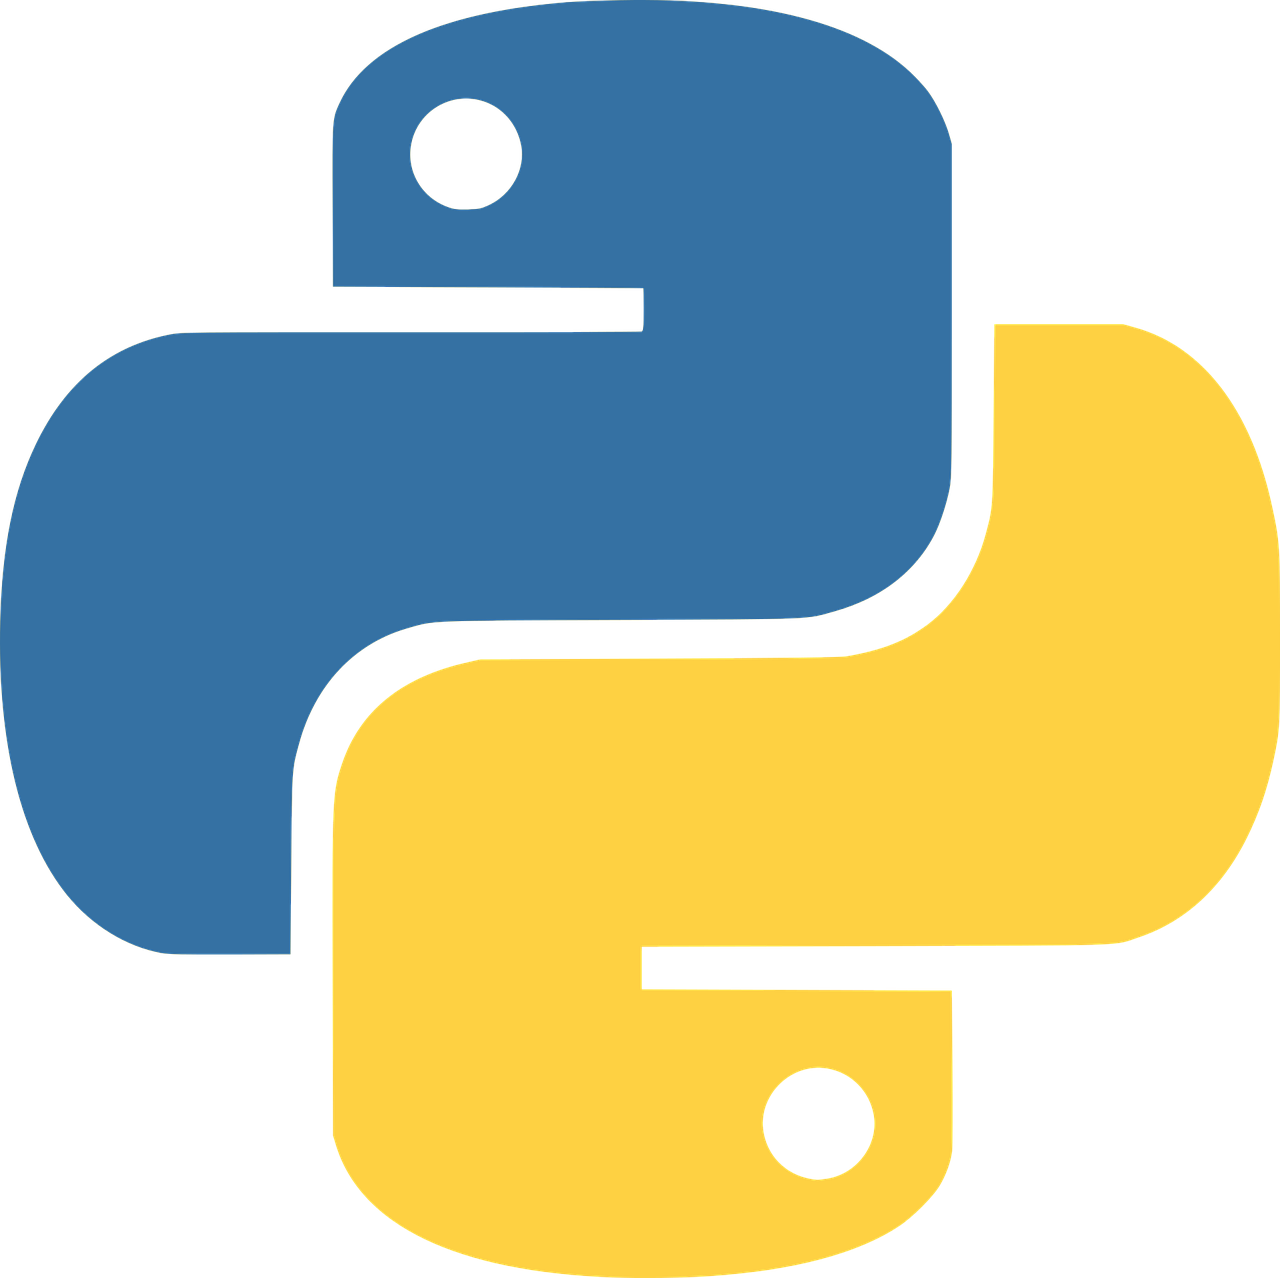
\includegraphics[scale=0.1]{python.png}
        \vspace{20pt}
\end{center}

\tableofcontents

\hypersetup{linkcolor=blue}

\newpage
\section*{Intro}

Je rédige ce doc \marginpar{\href{http://python.pycolore.fr}{Permalien}}au fur et à mesure que j'en apprends sur Python... Bonne lecture! (On peut rêver, peut-être ne suis-je pas le seul à le lire.)\bigskip

Ne sont pas reprises les opérations \og basiques \fg{} (boucles, manipulation des listes). On s'intéresse directement à la programmation orientée objet. Ensuite sont détaillés quelques fonctionnalités apportées par des modules. Une partie sur Django est particulièrement plus développée.\bigskip

Sauf exception, on considère qu'on travaille sur une distribution GNU/Linux (par exemple: Ubuntu, Fedora, Solus, Debian, Arch Linux).\bigskip

De nombreux liens sont disponibles. De manière générale:
\begin{enumerate}
    \item Des liens vers les documentations sont fournis.
    \item Des liens plus précis sont fournis en cliquant sur les termes dans la marge. <-- En cours! (càd incomplet)
    \item Pour le reste, tout ce qui est en bleu = lien (sauf dans les cadres de code).
\end{enumerate}

\paragraph{Nota Bene} Ce document est encore incomplet, des sections sont susceptibles d'être vides.

\newpage
\part{Programmation orientée objet en Python}

\section{Constantes et types natifs}
 Quelques constantes sont définies par Python comme \mintinline{python}{True}\index{True} et \mintinline{python}{False}\index{False}. De la même manière, quelques classes sont définies par défaut, appeléss types natifs, comme:

\begin{enumerate}
		\item Types booléennes
		\begin{enumerate}
			\item Booléen (\href{https://docs.python.org/fr/3/library/functions.html?highlight=bool#bool}{\mintinline{python}{bool}})
			\item Opérations booléennes (\href{https://docs.python.org/fr/3/library/stdtypes.html#boolean-operations-and-or-not}{\mintinline{python}{and, or, not}})
		\end{enumerate}
        \item Types numériques
        \begin{enumerate}
              \item Entier (\href{https://docs.python.org/fr/3/library/stdtypes.html#typesnumeric}{\mintinline{python}{int}})
              \item Flottant (\href{https://docs.python.org/fr/3/library/stdtypes.html#typesnumeric}{\mintinline{python}{float}})
              \item Complexe (\href{https://docs.python.org/fr/3/library/stdtypes.html#typesnumeric}{\mintinline{python}{complex}})
      \end{enumerate}
     \item Types séquentiels
	\begin{enumerate}
       \item Liste (\href{https://docs.python.org/fr/3/library/stdtypes.html#sequence-types-list-tuple-range}{\mintinline{python}{list}})
		\item Tuple (\href{https://docs.python.org/fr/3/library/stdtypes.html#sequence-types-list-tuple-range}{\mintinline{python}{tuple}})
		\item Range (\href{https://docs.python.org/fr/3/library/stdtypes.html#sequence-types-list-tuple-range}{\mintinline{python}{range}})
	\end{enumerate}
        \item Chaîne de caractères (\href{https://docs.python.org/fr/3/library/string.html?highlight=str#module-string}{\mintinline{python}{str}})
		\item Séquences binaires (\href{https://docs.python.org/fr/3/library/stdtypes.html#binary-sequence-types-bytes-bytearray-memoryview}{\mintinline{python}{bytes, bytearray, memoryview}})
		\item Ensemble (\href{https://docs.python.org/fr/3/library/stdtypes.html#set-types-set-frozenset}{\mintinline{python}{set}} (muable), \href{https://docs.python.org/fr/3/library/stdtypes.html#set-types-set-frozenset}{\mintinline{python}{frozenset}} (non muable))
		\item Dictionnaire (\href{https://docs.python.org/fr/3/library/stdtypes.html#mapping-types-dict}{\mintinline{python}{dict}})
\end{enumerate}

La liste n'est pas exhaustive, des compléments sur les types natifs sont disponibles dans la documentation.

\paragraph{Documentation} Documentation Python 3: \href{https://docs.python.org/fr/3/library/constants.html}{constantes natives}, \href{https://docs.python.org/fr/3/library/stdtypes.html}{types natifs}
%
% \section{Variables}
% \index{variable}

\section{Classes}
\index{classe}

 Les classes permettent des créer des objets\index{objet} appelés instances\index{instance}) qui partagent des caractéristiques de leur classe. Une classe correspond donc à un type, ou plutôt à un gabarit d'objet.

\paragraph{Documentation} \href{https://openclassrooms.com/courses/apprenez-a-programmer-en-python/premiere-approche-des-classes}{Introduction OpenClassrooms}, \href{https://docs.python.org/fr/3/tutorial/classes.html}{Documentation Python 3}, \href{https://fr.wikibooks.org/wiki/Programmation_Python/Classes#Définition_d'une_classe_élé mentaire}{Wikilivres}

\subsection{Structure d'une classe}
Les objets d'une classe partagent des caractéristiques communes à la classe: des attributs\index{attribut} et des méthodes (des fonctions qui agissent sur leur attributs). Les objets sont créés g\^ace à une méthode spéciale appelée constructeur.

\subsubsection{Création}
Pour créer une classe, la syntaxe est la suivante:
\begin{minted}{python}
class MaClasse:
    pass
\end{minted}

Si la classe hérite d'une classe mère, alors il faut l'ajouter en argument:
\begin{minted}{python}
class MaClasse(ClasseMere):
    pass
\end{minted}

\subsubsection{Initialiseur}
\index{initialiseur}\index{__init__}

L'initialiseur est une méthode spéciale appelée \Verb[fontsize = \small]|__init__|, il prend en argument \mintinline{python}{self}\index{self} (toutes les méthodes de la classe prennent en argument \mintinline{python}{self} qui est en fait l'instance en question) et tous les paramètres nécessaires à l'initialisation de l'instance. Il ne s'agit pas du constructeur (même si on l'appelle parfois ainsi par abus de langage) : il ne crée  pas à proprement parler l'instance, mais agit sur celle-ci lorsqu'elle vient d'être créée. Le \og véritable \fg{} constructeur est la méthode \mintinline{python}{__new__}, il n'est en général pas nécessaire de l'implémenter, sauf par exemple lorsque l'on crée des \hyperref[sec:metaclasses]{métaclasses} ou si l'on veut créer des classes qui héritent des types natifs. L'initialiseur est appelé automatiquement lors que l'on crée l'objet (après le constructeur).
\begin{minted}{python}
class MaClasse:
    CONSTANTE = ...
    def __init__(self, att1, att2):
        """Initialiseur"""
        self.attribut_1 = att1
        self.attribut_2 = att2
        self.attribut_3 = MaClasse.CONSTANTE
\end{minted}
Ici, les deux premiers attributs sont personnalisables lors de la création des objets alors que le dernier est commun à tous. \mintinline{python}{MaClasse.CONSTANTE} est une variable de classe\index{variable de classe}. Pour créer un objet on écrit simplement:
\begin{minted}{python}
objet = MaClasse(att1, att2)
\end{minted}

\subsubsection{Méthodes}
\index{méthode}
Les méthodes se définissent comme des fonctions, elles agissent en général sur les instances de la classe. Elles doivent prendre \mintinline{python}{self} en argument :
\begin{minted}{python}
class MaClasse:
    def __init__(self):
         pass

    def methode(self, arg1, arg2):
         pass
\end{minted}

Ensuite on les appelle de la manière suivante:
\begin{minted}{python}
objet.methode(arg1, arg2)
\end{minted}


\subsection{Héritage}
\index{héritage}

\subsubsection{Principe}

L'héritage est un moyen de créer des classes dérivées (classes filles) d'une classe source (classe mère). Une classe fille hérite de toutes les méthodes et variables de sa classe mère. Pour créer une classe fille, on utilise la syntaxe suivante.

\begin{minted}{python}
class Mere:
    pass

class Fille(Mere):
    pass
\end{minted}

Il est possible d'écraser une méthode héritée en la redéfinissant dans la classe fille. Si on veut accéder à une méthode héritée alors qu'on l'a redéfinie dans la classe fille, on utilise la fonction \mintinline{python}{super()} qui permet d'appeler la méthode de la classe mère de la classe présente (sans l'argument self).

\paragraph{Exemple}
\begin{minted}{python}
class Meuble:
    def __init__(self, couleur, materiau):
        self.couleur = couleur
        self.materiau = materiau

class Bibliotheque(Meuble):
    def __init__(self, couleur, materiau, n):
        super().__init__(couleur, materiau)
        self.nb_livres = n
\end{minted}
On peut utiliser deux fonctions pour vérifier l'héritage: \mintinline{python}{isinstance} renvoie \mintinline{python}{True} si l'objet est une instance de la classe ou de ses classes filles ; \mintinline{python}{issubclass} permet de voir si une classe est fille d'une autre.

\begin{Verbatim}[frame=single, fontsize=\footnotesize]
>>> bibli = Bibliotheque('blanc', 'vert', 150)
>>> bibli.__dict__
{'couleur': 'blanc', 'materiau': 'vert', 'nb_livres': 150}
>>> isinstance(bibli, Meuble)
True
>>> isinstance(bibli, Bibliotheque)
True
>>> issubclass(Bibliotheque, Meuble)
True
>>> issubclass(Meuble, Bibliotheque)
False
>>> isinstance(bibli, int)
False
>>> isinstance(bibli, object)
True
\end{Verbatim}

\paragraph{Documentation} \href{https://openclassrooms.com/courses/apprenez-a-programmer-en-python/l-heritage-9}{OpenClassrooms}, \href{https://docs.python.org/fr/3/tutorial/classes.html?highlight=héritage#inheritance}{Documentation Python 3}, \href{https://www.programiz.com/python-programming/inheritance}{Programiz}


\subsubsection{Ordre de résolution de méthode}

\subsubsection{Classe mère \mintinline{python}{object}}


\subsection{Propriétés}
\label{sec:proprietes}\index{propriété}\index{accesseur}\index{mutateur}\index{destructeur}
 Les propriétés représentent en Python le principe d'encapsulation. Elles sont utiles si on souhaite contrôler l'accès à un attribut ou si on veut que le changement d'une valeur d'un attribut engendre des modifications sur d'autres attributs. Les propriétés sont un cas particulier des descripteurs.

\subsubsection{Définition d'une propriété}

On crée les propriétés en utilisant des décorateurs. Elles contiennent un accesseur, un mutateur, un destructeur et une aide (docstring de l'accesseur).\bigskip

Les propriétés sont aussi un moyen de simuler des attributs privés: pour simuler un attribut privé, on précède son nom d'un souligné. Ainsi, on appelle cet attribut sans le souligné dans le code grâce aux propriétés. Par convention, on n'agit pas sur les attributs qui commencent par un souligné en Python.

\paragraph{Exemple}~
\begin{minted}{python}
class MaClasse:
    def __init__(self):
        self._attribut = 'Je suis un attribut'

    @property
    def attribut(self):
        """Propriété 'attribut'."""
        print("Accès à l'attribut")
        return self._attribut

    @attribut.setter
    def attribut(self, valeur):
        print("Modification de l'attribut")
        self._attribut = valeur

    @attribut.deleter
    def attribut(self):
        print('Adieu :(')
        del self._attribut
\end{minted}

On utilise la propriété de la manière suivante:
\begin{Verbatim}[frame=single, fontsize=\footnotesize]
>>> instance = MaClasse()
>>> instance.attribut
Accès à l'attribut
'Je suis un attribut'
>>> instance.attribut = 'Ah bon ?'
Modification de l'attribut
>>> del instance.attribut
Adieu :(
>>> help(MaClasse.attribut)
Help on property:

    Propriété 'attribut'.

\end{Verbatim}

\paragraph{Documentation}\href{https://docs.python.org/fr/3/library/functions.html?highlight=property#property}{Documentation Python 3}, \href{https://stackoverflow.com/questions/15750522/class-properties-and-setattr/15751159#15751159}{Priorités entre propriété et méthodes spéciales}
\subsubsection{Généralisation: les descripteurs}
On dit qu'un objet est un descripteur s'il possède au moins une méthode \mintinline{python}{__get__} (accesseur), \mintinline{python}{__set__} (mutateur), ou \mintinline{python}{__delete__} (destructeur).

\paragraph{Exemple} Exemple d'implémentation
\begin{minted}{python}
class Attribut:
    def __get__(self, inst, insttype):
        print("Accès à l'attribut")
        return inst._attribut

    def __set__(self, inst, valeur):
        print("Modification de l'attribut")
        inst._attribut = valeur

class MaClasse:
    def __init__(self):
        self._attribut = 'Je suis un attribut'

    attribut = Attribut()
\end{minted}

\paragraph{Documentation} \href{https://docs.python.org/3/howto/descriptor.html}{Documentation Python 3}



\subsection{Méthodes statiques et méthodes de classes}
\subsubsection{Méthode statique}
\index{méthode statique}
Les méthodes que l'on a vues jusqu'à maintenant agissent sur les instances des classes : elles prennent toujours en premier argument le mot clé \mintinline{python}{self} qui renvoie à l'instance elle même. Lorsque l'on appelle une telle méthode sur une instance comme ceci:
\mintinline[fontsize=\small]{python}
{instance.methode(<arguments>)},
Python exécute en fait \mintinline{python}{Classe.methode(instance, <arguments>)}.\bigskip

En fait, ces deux objets sont différents. \mintinline{python}{Classe.methode} est une simple fonction, alors que \mintinline{python}{instance.methode} est une méthode évaluée sur l'instance (en anglais \og bound method \fg{}\index{bound method}), c'est-à-dire que l'instance est mise en premier argument. On considère cet exemple:

\paragraph{Exemple}
\begin{minted}{python}
class Maths:

    def addition(x, y):
        return x + y

    def multiplication(x, y):
        return x * y

    def division(x, y):
        return x / y
\end{minted}
On choisit ici de grouper trois fonctions car elles sont logiquement liées. Elles n'influent pas les instances donc elles ne prennent pas \mintinline{python}{self} en argument. Si l'on appelle ces méthodes sur une instance, une exception sera levée car Python entrera automatiquement l'argument \mintinline{python}{self} (donc en tout trois arguments) alors que les méthodes n'en prennent que deux. Pour remédier à cela, on les décore avec \mintinline{python}{@staticmethod}. On peut maintenant les appeler indifféremment sur la classe ou sur des instances.

\subsubsection{Méthode de classe}
\index{méthode de classe}\label{sec:classmethod}
Lorsque l'on veut manipuler des variables de classe et non des attributs d'instances, on crée des méthodes de classe. Celles-ci prennent la classe en premier argument, par convention on le note \mintinline{python}{cls}; elles ne prennent logiquement pas \mintinline{python}{self} comme argument. Cette méthode est donc évaluée sur la classe. Sans autre modification, on ne peut peut appeler cette méthode que sur les instances car Python attend l'argument \mintinline{python}{cls}. Pour pouvoir appeler cette méthode sur la classe (logique car c'est une méthode de classe), on la décore avec \mintinline{python}{@classmethod}.

\subsubsection{Cas de l'héritage}
En résumé:
\begin{enumerate}
        \item Les méthodes statiques sont des fonctions reliées à des classes, mais qui n'agissent pas sur celles-ci.
        \item Les méthodes de classe sont des fonctions qui prennent la classe en paramètre.
\end{enumerate}

Une classe qui hérite d'une classe mère hérite de toutes ses méthodes. Les méthodes statiques restent donc inchangées, tandis que les méthodes de classe s'adaptent à la nouvelle classe, car elles la prennent en premier argument.

\paragraph{Exemple} Un exemple d'utilisation de méthodes statiques et de classe sont la création de constructeurs alternatifs. On s'aperçoit de la différence des deux notions.
\begin{minted}{python}
class Personne:
    def __init__(self, nom, age):
        self.nom = nom
        self.age = age

    @staticmethod
    def par_date_de_naissance(nom, date):
        return Personne(nom, 2018-date)

    @classmethod
    def par_date_de_naissance2(cls, nom, date):
        return cls(nom, 2018-date)

class Homme(Personne):
    sexe = 'homme'
\end{minted}
\begin{Verbatim}[frame=single, fontsize=\footnotesize]
>>> homme1 = Homme.par_date_de_naissance('Jean', 1997)
>>> homme2 = Homme.par_date_de_naissance2('Jean', 1997)
>>> type(homme1)
<class '__main__.Personne'>
>>> type(homme2)
<class '__main__.Homme'>
\end{Verbatim}

Pour avoir \mintinline{python}{homme1} de type \mintinline{python}{Homme}, il faut redéfinir la méthode statique dans la classe fille.

\paragraph{Documentation} \href{https://www.programiz.com/python-programming/methods/built-in/staticmethod}{Méthode statique sur Programiz}, \href{https://www.programiz.com/python-programming/methods/built-in/classmethod}{Méthode de classe sur Programiz}, \href{https://stackoverflow.com/questions/136097/what-is-the-difference-between-staticmethod-and-classmethod-in-python/1669524#1669524}{StackOverflow}



\subsection{Méthodes spéciales}
\index{méthode spéciale}
 Les méthodes spéciales sont déjà définies par défaut dans Python mais on peut les personnaliser. Elles sont reconnaissables par leur typographies: leur nom commence et se termine par deux soulignés. On en introduit quelques unes seulement ici.

\paragraph{Documentation} \href{https://docs.python.org/3/reference/datamodel.html#specialnames}{Documentation Python 3}, \href{https://openclassrooms.com/courses/apprenez-a-programmer-en-python/les-methodes-speciales-1}{OpenClassrooms}


\subsubsection{Construction, initialisation et destruction}
Le constructeur est la méthode \mintinline{python}{__new__}. C'est une \hyperref[sec:staticmethod]{méthode statique} qui prend en argument la classe de l'objet à instancier (\mintinline{python}{cls}) et les autres arguments qui seront en paramètres de l'initialiseur; il doit retourner un objet (l'instance à créer). \mintinline{python}{__init__} a déjà été décrit précédemment (contrairement au constructeur, cette méthode ne retourne rien). En pratique, on n'implémente pas la méthode \mintinline{python}{__new__} sauf dans certains cas.

\paragraph{Exemple} On veut définir une classe \og singleton \fg{} qui ne peut créer qu'une instance.

\begin{minted}{python}
class Singleton:
    """Classe qui ne peut instancier qu'une fois."""

    instance = None

    def __new__(cls, *args, **kwargs):
        if not cls.instance:
            cls.instance = super().__new__(cls)
            return cls.instance
        else:
            raise TypeError(r"Cette classe singleton possède déjà une instance : {cls.instance}")

    def __del__(self):
        Singleton.instance = None

    def __init__(self, *args, **kwargs):
        pass
\end{minted}

Pour détruire un objet, on définit la méthode \mintinline{python}{__del__}\index{__del__}. On l'appelle comme ceci:
\begin{minted}{python}
del objet
\end{minted}

\subsubsection{Représentation et chaine de caractère d'un objet}
Il existe deux méthodes spéciales nommées \mintinline{python}{__repr__}\index{__repr__} et \mintinline{python}{__str__}\index{__str__} qui sont appelées lorsque l'on exécute \mintinline{python}{repr(objet)} ou \mintinline{python}{return objet}, et quand on exécute \mintinline{python}{str(objet)} ou bien \mintinline{python}{print(objet)}. La fonction \mintinline{python}{__repr__} est donc utilisée lorsque l'on veut avoir accès à la représentation d'un objet, tandis que \mintinline{python}{__str__} permet de présenter l'objet de manière plus élégante en chaîne de caractères. Ces deux fonctions prennent en argument \mintinline{python}{self}. Lorsque la méthode \mintinline{python}{__str__} n'est pas définie, Python appelle la fonction de représentation à la place.

\paragraph{Exemple} L'exemple suivant
\begin{minted}{python}
class MaClasse:
    def __init__(self):
         self.attribut = 'Exemple'

    def __repr__(self):
        return "MaClasse({})".format(self.attribut)

    def __str__(self):
        return "Instance de MaClasse ayant comme attribut {}"
              .format(self.attribut)
\end{minted}
permet de faire:
\begin{Verbatim}[frame=single, fontsize=\footnotesize]
>>> obj = MaClasse()
>>> obj
MaClasse(Exemple)
>>> print(obj)
Instance de MaClasse ayant comme attribut Exemple.
\end{Verbatim}

\subsubsection{Accesseur et mutateur}
\index{accesseur}\index{mutateur}\index{destructeur}
Lorsque Python essaie d'accéder à un attribut, il appelle en premier la méthode spéciale \mintinline{python}{__getattribute__}\index{__getattribute__}, puis il appelle les \hyperref[sec:proprietes]{descripteurs} s'il sont définis. Lorsque l'on veut modifier un attribut, c'est la méthode spéciale \mintinline{python}{__setattr__}\index{__setattr__} puis les descripteurs qui sont appelés. Si on essaie d'accéder à un attribut non défini, Python appelle en guise de dernière chance la méthode \mintinline{python}{__getattr__}\index{__getattr__}. On peut personnaliser cette fonction de manière à ce qu'elle envoie une erreur, ou bien à ce qu'elle redirige vers un autre attribut ou effectue un calcul.

\paragraph{Exemple}
\begin{minted}{python}
class MaClasse:
    def __init__(self)
        self.a = int()

    def __getattribute__(self, attribut):
        print("J'accède à l'attribut {}...".format(attribut))
        return object.__getattribute__(self, attribut)

    def __getattr__(self, attribut):
        print("L'attribut {} est inaccessible !".format(attribut))

    def __setattr__(self, attribut, valeur):
        object.__setattr__(self, attribut, valeur)
        print("L'attribut a été changé !")
        # Il est nécessaire d'appeler la méthode par défaut, car appeler self.__setattr__
        # donnerait une récursivité infinie. En fait, on ne sait à ce stade pas comment
        # Python change concrètement la valeur de l'attribut.
\end{minted}

On note que l'on utilise les méthodes spéciales de la classe \mintinline{python}{object} (méthodes par défaut) car appeler \mintinline{python}{self.__getattribute__} ou \mintinline{python}{self.__setattr__} donnent une récursivité sans fin ! Cela permet de faire:
\begin{Verbatim}[frame=single, fontsize=\footnotesize]
>>> objet = MaClasse()
L'attribut a été changé !
>>> objet.b
L'attribut b est inaccessible !
>>> objet.a
J'accède à l'attribut a...
0
>>> objet.attribut = 1
L'attribut a été changé !
>>> objet.a
J'accède à l'attribut a...
1
\end{Verbatim}
Il existe aussi \mintinline{python}{__delattr__}\index{__delattr__} qui prend en arguments \mintinline{python}{self} et le nom de l'attribut. Cette méthode est appelée lorsque l'on effectue \mintinline{python}{del objet.attribut}. Lors de l'écriture de la méthode, il faut utiliser \mintinline{python}{object.__delattr__} de la même manière que l'on utilise \mintinline{python}{object.__setattr__} pour \mintinline{python}{__setattr__} ou \mintinline{python}{object.__getattribute__} pour \mintinline{python}{__getattribute__}.\bigskip

\subsubsection{Surcharges d'opérateur}
\index{surcharge d'opérateur}
Les surcharges d'opérateur permettent de faire des opérations arithmétiques avec des objets, c'est-à-dire d'indiquer à Python ce qu'il faut faire lorsque l'on exécute \mintinline{python}{objet1 + objet2}. Ces méthodes prennent en arguments \mintinline{python}{self} (l'objet 1) et l'objet 2.
\begin{center}
\begin{tabular}{|p{2.5cm}|c|}
        \hline
        \multicolumn{1}{|c|} {\bf Méthode} & {\bf Appel}\\
        \hline
        \mintinline{python}{__add__}\index{__add__} & \mintinline{python}{objet1 + objet2}\\
        \hline
        \mintinline{python}{__sub__}\index{__sub__} & \mintinline{python}{objet1 - objet2}\\
        \hline
        \mintinline{python}{__mul__}\index{__mul__} & \mintinline{python}{objet1 * objet2}\\
        \hline
        \mintinline{python}{__truediv__}\index{__truediv__} & \mintinline{python}{objet1 / objet2}\\
        \hline
        \mintinline{python}{__floordiv__}\index{__floordiv__} & \mintinline{python}{objet1 // objet2}\\
        \hline
        \mintinline{python}{__mod__}\index{__mod__} & \mintinline{python}{objet1 \% objet2}\\
        \hline
\end{tabular}
\end{center}
Les deux objets ne sont pas nécessairement du même type ! Cependant, cette opération n'est pas symétrique : le code \mintinline{python}{objet + 5} par exemple exécute \mintinline{python}{objet.__add__(5)}, alors que \mintinline{python}{5 + objet} exécute \mintinline{python}{int.__add__(5)}. Pour que l'opération soit symétrique, il faut aussi définir ces fonctions avec le préfixe \mintinline{python}{r} (par exemple \mintinline{python}{__radd__}).

\section{Fonctions et objets exécutables}
La façon la plus basique de définir une fonction est d'utiliser le mot-clé \mintinline{python}{def}. Lorsque l'on appelle, on spécifie des arguments aux paramètres de la fonction.

\begin{minted}{python}
fonction(argument_de_paramètre_non_nommé, paramètre_nommé=argument)
\end{minted}

On peut utiliser les opérateurs d'\emph{unpacking} (\og déballage \fg{}) :
\begin{itemize}
    \item Lorsque l'on écrit les paramètres pour capter tous les paramètres possibles.
    \item Pour renseigner les arguments.
\end{itemize}

\paragraph{Exemple}
\begin{minted}{python}
# Cette fonction accepte tous les arguments
def fonction(*args, **kwargs):
    pass

# Celle-ci en accepte 4. On va tester sur celle-ci l'unpacking.
def fonction(par1, par2, par3, par4):
    for (arg, value) in locals().items():
        print(arg, ':', value)

arg1, arg2, arg3, arg4 = 1, 2, 3, 4
tuple_args = (arg1, arg2)
dict_args = {'par3': arg3, 'par4': arg4}

# Testons l'unpacking
fonction(*tuple_args, **dict_args)

# Sortie
# par4 : 4
# par3 : 3
# par2 : 2
# par1 : 1
\end{minted}

\section{Conteneurs}

\paragraph{Remarque préléminaire} Pour les méthodes spéciales spécifiques aux types des parties suivantes, je me base sur le module \hyperref[abc]{\mintinline{python}{collections.abc}}\bigskip


Les conteneurs sont des objets voués à contenir d'autres objets. Les principaux exemples de conteneurs sont les listes, les chaînes de caractères, les tuples, les dictionnaires ou encore les ensembles. Un objet est dit conteneur s'il possède la méthode spéciale \mintinline{python}{__contains__()}.

\begin{description}
    \item[\mintinline{python}{conteneur.__contains__(objet)}]~

    Retourne \mintinline{python}{True} si \mintinline{python}{objet} est présent dans \mintinline{python}{conteneur}, \mintinline{python}{False} sinon. On appelle cette méthode spéciale comme ceci:
    \begin{minted}{python}
objet in conteneur
    \end{minted}
\end{description}

\paragraph{Remarque} La fonction \mintinline{python}{__contains__()} est définie chez les itérateurs, mais ceux-ci ne sont pas pas des conteneurs ! Implémenter cette méthode n'est donc pas une condition suffisante pour qu'un objet soit un conteneur (voir la section sur les \hyperref[iterateur]{itérateurs}).\bigskip

La plupart des conteneurs possède une taille. Elle calculée par la méthode spéciale \mintinline{python}{__len__()}.
\begin{description}
    \item[\mintinline{python}{conteneur.__len__()}]~

    Retourne la taille du conteneur. Devrait retourner un entier positif ou nul. Si cette fonction retourne autre chose, une exception est levée. On l'appelle comme ceci:
    \begin{minted}{python}
len(conteneur)
    \end{minted}
\end{description}
\paragraph{Exemples} Des \og sized \fg{} capricieux
\begin{minted}{python}
class StrSized:
    def __len__(self):
        return 'Ma taille !'

class NegativeSized:
    def __len__(self):
        return -1

len(StrSized()) # TypeError: 'str' object cannot be interpreted as an integer
len(NegativeSized()) # ValueError: __len__() should return >= 0
\end{minted}

Notons qu'un objet peut avoir une taille sans pour autant être un conteneur (on appelle ça un \emph{sized}).

\subsection{Conteneurs indexables}
Parmi ces conteneurs se distinguent les conteneurs que l'on peut indexer. Ce sont les conteneurs sur lesquels on peut utiliser les crochets \mintinline{python}{[]} pour faire référence à un objet dans le conteneur; on parle de table de correspondance (\emph{mapping}, non détaillé ici), et de séquence lorsque les index sont des entiers. Parmi les exemples cités précédemment, seuls les ensembles ne sont pas indexables. On rend un objet indexable en implémentant une méthode spéciale.

\begin{description}
    \item[\mintinline{python}{indexable.__getitem__(index)}]~

    Retourne l'objet référencé par \mintinline{python}{index} (cet indice peut être n'importe quel objet). Appelée en faisant:
    \begin{minted}{python}
indexable[index]
    \end{minted}
\end{description}

On peut rendre mutables les objets indexables grâce à deux méthodes spéciales.

\begin{description}
    \item[\mintinline{python}{indexable.__setitem__(index, valeur)}]~

    Assigne la nouvelle \mintinline{python}{valeur} à l'objet référencé par \mintinline{python}{index}. Appel:
    \begin{minted}{python}
indexable[index] = valeur
    \end{minted}

    \item[\mintinline{python}{indexable.__delitem__(index)}]~

    Détruit l'objet référencé par \mintinline{python}{index}. Appel:
    \begin{minted}{python}
del indexable[index]
    \end{minted}
\end{description}

\subsection{Objets séquentiels}

Les objets séquentiels sont des objets indexables qui n'acceptent que des entiers comme index. <a venir : Slices>


\section{Itérateurs}\label{iterateur}
\index{itérateur}

Les itérateurs sont des objets incontournables en Python, ils sont notamment utilisés lorsque l'on fait une boucle \mintinline{python}{for}. Les objets itérateurs peuvent être créés par des objets itérables. Des itérables connus sont les listes, les dictionnaires, les tuples, les \mintinline{python}{range()}.\bigskip

L'intérêt principal des itérateurs est leur faible consommation mémoire: contrairement à un objet conteneur qui prend autant d'espace que d'objets qu'il contient, un itérateur calcule chaque élément lorsqu'il est appelé.

\paragraph{Exemple} Ce qu'il se passe lorsque l'on fait une boucle \mintinline{python}{for}
\begin{minted}{python}
>>> L = [0, 1, 2, 3, 4] # les listes sont des objets itérables
>>> for element in L # appelle l'itérateur de l'itérable L
...    print(element) # à chaque ligne, appelle l'élément suivant de l'itérateur
0
1
2
3
4
\end{minted}

Les itérateurs sont implémentés sous forme de classes et doivent respecter le protocole d'itérateur: deux méthodes spéciales doivent être implémentées.
\begin{description}
    \item[\mintinline{python}{iterateur.__iter__()}]~

    Cette méthode retourne l'itérateur lui-même, on peut y effectuer quelques opérations d’initialisation. Appel:
    \begin{minted}{python}
iter(iterateur)
    \end{minted}

    \item[\mintinline{python}{iterateur.__next__()}]~

    Cette méthode retourne l'élément suivant dans la séquence de l'itérateur. Une fois que le dernier élément a été appelé, lève une exception \mintinline{python}{StopIteration}. Appel:
    \begin{minted}{python}
next(iterateur)
    \end{minted}
\end{description}

Les itérables doivent quant à eux implémenter la méthode \mintinline{python}{__iter__()} qui appelle l'itérateur associé. On l'appelle en faisant \mintinline{python}{iter(objet_iterable)}.

\paragraph{Exemple} Un incrémenteur
\begin{minted}{python}
class Incrementor:
    def __init__(self, max):
        self.max = max

    def __iter__(self):
        self. n = 0
        return self

    def __next__(self):
        if self.n <= self.max:
            result = self.n
            self.n += 1
            return result
        else:
            raise StopIteration
\end{minted}
On peut maintenant utiliser l'itérateur.
\begin{minted}{python}
>>> inc = Incrementor(2)
>>> iterator = iter(inc)
>>> next(inc)
0
>>> next(inc)
1
>>> next(inc)
2
>>> next(inc)
Traceback (most recent call last):
  File "<stdin>", line XX, in <module>
    print(next(iterator))
  File "<stdin>", line XX, in __next__
    raise StopIteration
StopIteration
\end{minted}
On peut aussi utiliser une boucle \mintinline{python}{for} pour itérer notre itérateur.
\begin{minted}{python}
>>> for i in Incrementor(5):
...    print(i)
0
1
2
3
4
5
\end{minted}

\section{Générateurs}
\index{générateur}
\subsection{Fonction génératrice et mot-clé \mintinline{python}{yield}}

Les générateurs sont une façon plus simple d'utiliser les itérateurs. Au lieu de créer une classe avec les deux méthodes du protocole d'itération, on définit une fonction qui retourne les résultats avec le mot clé \mintinline{python}{yield}. Lorsqu'une fonction possède ce mot-clé, l'appeler crée un générateur, et rien d'autre n'est exécuté. Un générateur est un itérateur auquel on peut ajouter des méthodes supplémentaires (cf. plus bas); ce sont en quelque sorte des itérateurs upgradés. On appelle par abus de langage les fonctions qui retournent des générateurs (des \og fonctions génératrices \fg{}) des générateurs aussi (alors que ce sont de simples fonctions).\bigskip

Pour faire le lien avec les itérateurs, on peut réécrire l'exemple précédent à l'aide d'un générateur.
\begin{minted}{python}
def incrementor(max):
    n = 0
    while n <= max:
        yield n
        n += 1
\end{minted}

On utilise les générateurs comme des itérateurs (les générateurs sont des itérateurs). Lorsque l'on évalue la méthode \mintinline{python}{__next__()} sur un générateur (en faisant \mintinline{python}{next(generateur)}), celui-ci parcourt la fonction génératrice jusqu'au premier \mintinline{python}{yield} qu'il rencontre, puis s'arrête. Lorsque la méthode \mintinline{python}{__next__()} est de nouveau appelée, le générateur continue le parcours jusqu'au \mintinline{python}{yield} suivant, et ainsi de suite. Lorsqu'il n'y en a plus, le générateur lève une exception \mintinline{python}{StopIteration}.
\begin{minted}{python}
>>> gen = incrementor(2)
>>> next(gen)
0
>>> next(gen)
1
>>> next(gen)
2
>>> next(gen) # Erreur
StopIteration
>>> for i in incrementor(2):
...    print(i)
0
1
2
\end{minted}

On n'appelle pas la méthode \mintinline{python}{iter()} sur un générateur. Ainsi, pour réinitialiser le générateur, on doit le recréer en appelant une nouvelle fois la fonction génératrice.

\subsection{Fonctions supplémentaires}
En plus du mot-clé \mintinline{python}{yield}, on peut utiliser des fonctions supplémentaires dans les générateurs:
\begin{description}
    \item[\mintinline{python}{generateur.send()}]~

    Cette méthode permet de communiquer avec l'itérateur en lui envoyant une valeur. Lorsqu'elle est appelée avec un argument, celui-ci est retourné par le \mintinline{python}{yield} actuellement atteint, et le générateur reprend le parcours jusqu'au \mintinline{python}{yield} suivant. Ainsi, appeler cette méthode consomme une itération ! C'est comme si l'on appelait \mintinline{python}{__next__()} en même temps.
\end{description}

Ainsi, l'instruction \mintinline{python}{yield} renvoie quelque chose, en plus de fournir au générateur la valeur suivante. Cela se passe dans cet ordre:
\begin{enumerate}
    \item On appelle \mintinline{python}{__next__()}, le générateur parcourt la fonction jusqu'au premier \mintinline{python}{yield}.
    \item Le générateur rencontre un \mintinline{python}{yield}. Il envoie ce que le \mintinline{python}{yield} lui fournit et se met en pause.
    \item Le générateur est à nouveau appelé. Si c'est avec un \mintinline{python}{send()}, il donne le paramètre du \mintinline{python}{send()} au \mintinline{python}{yield} qui le retourne à la variable à laquelle il est affectée.
    \item Une fois que c'est fait, le générateur reprend le parcours de la fonction jusqu'au \mintinline{python}{yield} suivant, (retour à l'étape 2).
\end{enumerate}

\paragraph{Exemple} On reprend l'incrémenteur et on veut pourvoir l'étendre, c'est à dire lui envoyer un nombre et l'ajouter au maximum initial. On modifie la fonction génératrice. On ajoute des \mintinline{python}{print()} pour voir comment fonctionne \mintinline{python}{send()}
\begin{minted}{python}
def incrementor(max):
    n = 0
    while n <= max:
        print(f"max_pre : {max}")
        add_max = yield n
        print(f"max_post : {max}")
        print(f"add_max : {add_max}")
        n += 1
        max = max + add_max if add_max else max
\end{minted}
Lorsque l'on appelle \mintinline{python}{send}, la valeur est stockée dans \mintinline{python}{add_max}. On peut alors étendre l'incrémenteur.
\begin{minted}{python}
>>> gen = incrementor(2)
>>> next(gen)   # Le générateur est appelé, il commence le parcours
max_pre : 2     # Il rencontre le premier print()
0               # et un yield : il envoie ce que celui-ci lui fournit...
>>> next(gen)   # et attend qu'on le rappelle !
max_post : 2    # il reprend son parcours
add_max : None  # on voit bien que l'on a rien envoyé au générateur
max_pre : 2
1
>>> next(gen)
max_post : 2
add_max : None  # toujours rien...
max_pre : 2
2
>>> gen.send(3) # Le yield retourne à add_max la valeur de send()
max_post : 2    # le générateur reprend le parcours...
add_max : 3     # On a bien un add_max de 3 !
max_pre : 5     # arrivé au while, le max a donc changé, la boucle peut donc continuer !
3               # et on atteint bien le yield suivant
>>> next(gen)
max_post : 5
add_max : None
max_pre : 5
4
\end{minted}
En fait, on s'aperçoit que \mintinline{python}{next(gen)} et \mintinline{python}{gen.send(None)} sont équivalents. On ne peut pas appeler \mintinline{python}{send()} avec autre chose que \mintinline{python}{None} en paramètre avant d'avoir appelé au moins une fois \mintinline{python}{__next__()}. En effet, l'affectation se fait par l'intermédiaire du \mintinline{python}{yield} actuel.

\begin{description}
    \item[\mintinline{python}{generateur.throw(type[, value, traceback])}]~

    Envoie une exception au générateur. Si celui-ci l'attrape, alors retourne également la valeur suivante du générateur.

    \item[\mintinline{python}{generateur.close()}]~

    Envoie une exception au générateur
\end{description}

\section{Décorateurs}
\index{décorateur}
Les décorateurs sont des fonctions ou des classes qui permettent de modifier le comportement d'une autre fonction (ou classe). Les décorateurs sont utiles lorsque l'on souhaite qu'un certain nombre de fonctions effectuent des tâches communes comme par exemple donner leur temps d'exécution. On appelle un décorateur de la manière suivante.

\begin{minted}{python}
@decorateur
def fonction():
    pass
\end{minted}

Le code précédent a le même comportement que le code suivant.

\begin{minted}{python}
def fonction():
    pass

fonction = decorateur(fonction)
\end{minted}

Ainsi, \mintinline{python}{fonction} devient l'objet retournée par \mintinline{python}{decorateur(fonction)}. Le décorateur doit donc retourner un objet que l'on peut appeler en écrivant \mintinline{python}{objet()} (avec d'éventuels arguments), on appelle ce type d'objet un \og exécutable\fg{}\index{exécutable}. Le décorateur est bien sûr lui même un exécutable. Si on le définit comme une classe, on doit définir la méthode \mintinline{python}{__call__} qui permet de rendre ses instances exécutables.

\paragraph{Documentation} \href{https://stackoverflow.com/questions/739654/how-to-make-a-chain-of-function-decorators/1594484#1594484}{Stack Overflow}

\subsection{En tant que classe}
Une façon d'implémenter un décorateur est d'utiliser les classes. La fonction décorée deviendra alors une instance de la classe de ce décorateur. Il faut obligatoirement définir la méthode \mintinline{python}{__call__} pour pouvoir rendre cette instance exécutable.

\paragraph{Exemple} On considère ici un décorateur qui compte le nombre d'appels de la fonction décorée.
\begin{minted}{python}
class Compteur:
    def __init__(self, f):
        self.call = 0
        self.f = f

    def __call__(self, *args, **kwargs):
        self.call += 1
        print("La fonction {} a été appelée {} fois.".format(self.f.__name__, self.call))
        return self.f(*args, **kwargs)
\end{minted}
\subsection{En tant que fonction}
Comme un décorateur est un objet exécutable qui n'a d'autre utilité que d'être appelé, il est aussi logique de le définir en tant que fonction.

\paragraph{Exemple} Même décorateur que précédemment mais en l'implémentant en tant que fonction.
\begin{minted}{python}
def compteur(f):
    def wrapper(*args, **kwargs):
        wrapper.call += 1
        print("La fonction {} a été appelée {} fois.".format(f.__name__, wrapper.call))
        return f(*args, **kwargs)
    wrapper.call = 0
    return wrapper
\end{minted}
\paragraph{Remarques} On voit dans cet exemple que l'on peut définir des fonctions dans les définitions de fonctions. La mention \mintinline{python}{*args} fait référence à tous les arguments non nommés que l'on a entrés (c'est un tuple, par exemple \mintinline{python}{(arg1, arg2)}). La mention \mintinline{python}{**kwargs} fait référence aux arguments nommés (c'est un dictionnaire). Ainsi on est sûr de récupérer tous les arguments.\bigskip

Dans cet exemple, on assigne à \mintinline{python}{wrapper} un attribut de fonction (on peut le faire, puisqu'une fonction est un objet -- de la classe \mintinline{python}{function}). On le définit après avoir défini cette fonction.

\subsection{Décorateurs à paramètres}
On peut faire en sorte que le décorateur prenne un ou plusieurs paramètres. Dans ce cas, il faut définir le décorateur à l'intérieur d'une clôture qui prend en argument ces différents paramètres.

\paragraph{Exemple} On veut retourner une erreur quand la fonction retourne une valeur trop élevée.
\begin{minted}{python}
def depasse_max(max):
    def deco(f):
        def wrapper(*args, **kwargs):
            n = f(*args, **kwargs)
            if n > max:
                print("Maximum {} dépassé.".format(max))
                return
            return n
        return wrapper
    return deco
\end{minted}

Ces deux syntaxes sont équivalentes:

\begin{minted}{python}
@depasse_max(10)
def demande_nombre():
    n = int(input("Entrer un nombre : "))
    return n

def demande_nombre():
    n = int(input("Entrer un nombre : "))
    return n

demande_nombre = depasse_max(10)(demande_nombre)
\end{minted}

Cela permet de faire

\begin{Verbatim}[frame=single, fontsize=\footnotesize]
>>> demande_nombre()
Entrer un nombre : 11
Maximum 10 dépassé.
\end{Verbatim}

\section{Métaclasses}
\subsection{Principe}
\index{métaclasse}\label{sec:metaclasses}
Les métaclasses sont les classes qui instancient d'autres classes. Par défaut, une seule métaclasse est définie : la métaclasse \mintinline{python}{type}. On s'en rend compte en demandant le type des classes que l'on crée.

\begin{minted}{python}
class MaClasse:
    pass

print(type(MaClasse)) # <class 'type'>
\end{minted}

\subsection{La métaclasse \mintinline{python}{type}}

\subsection{Application pythonique: propriété de classe}
On pourrait imaginer des propriétés de classes afin d'ajouter une couche de logique sur une simple variable de classe. Au lieu de définir un descripteur générique, on créer une métaclasse qui aura comme popriété la future propriété de classe.

\paragraph{Exemple} Un exemple simple
\begin{minted}{python}
class MaMetaclasse(type):
    @property
    def propriete(self):
        return self._propriete
    @propriete.setter
    def propriete(self, value):
        self._propriete = value

class MaClasse(metaclass=MaMetaclasse):
    _propriete = 5

print(MaClasse.propriete) #5
\end{minted}

\newpage

\part{Librairie standard}

\section{Classes abstraites : abc, collections.abc}\label{abc}

\section{re}
\index{re}\index{expression régulière}
Le module \mintinline{python}{re} permet d'utiliser les expressions régulières en Python.
\paragraph{Documentation} \href{https://docs.python.org/fr/3/library/re.html}{Documentation Python 3}

\subsection{Ecrire une expression régulière}
Les expressions régulières sont un excellent moyen de retrouver des motifs complexes dans une chaîne de caractères. On écrit les motifs à rechercher grâce à plusieurs caractères spéciaux:
\begin{description}
    \item [Spécification du caractère]~
    \begin{itemize}
        \item \og\mintinline{text}{.}\fg{} désigne n'importe quel caractère.
        \item \og\mintinline{text}{[]}\fg{} permet de dire quels caractères on veut trouver (\mintinline{text}{[a-e]} : \mintinline{text}{a}, \mintinline{text}{b}, \mintinline{text}{c}, \mintinline{text}{d} ou \mintinline{text}{e}; \mintinline{text}{[a-eA-E]} idem avec les majuscule comprises; \mintinline{text}{[+-*]}: soit \mintinline{text}{*} soit \mintinline{text}{+} soit \mintinline{text}{-}).
        \item \og\Verb[fontsize=\small]|\w|\fg{} équivaut à \Verb[fontsize=\small]|[a-zA-Z0-9_]|.
        \item \og\Verb[fontsize=\small]|\W|\fg{} désigne tout caractère non alpha-numérique.
        \item \og\Verb[fontsize=\small]|\d|\fg{} équivaut à \mintinline{text}{[0-9]}.
        \item \og\Verb[fontsize=\small]|\D|\fg{} désigne tout caractère non numérique.
        \item \og\Verb[fontsize=\small]|\s|\fg{} désigne un espace.
    \end{itemize}
    \item [Place du motif dans la chaine]~
    \begin{itemize}
        \item \og\Verb[fontsize=\small]!^!\fg{} (se place au début) signifie que le début de la chaine doit correspondre au motif.
        \item \og\mintinline{text}{\$}\fg{} (se place à la fin) signifie que la fin de la chaine doit correspondre au motif.
    \end{itemize}
    \item [Nombre d'apparition(s) consécutive(s)]~
    \begin{itemize}
        \item \og\mintinline{text}{\{n\}}\fg{} indique que le caractère précédent doit apparaitre \mintinline{text}{n} fois.
        \item \og\mintinline{text}{\{n,m\}}\fg{} indique que le caractère précédent doit apparaitre entre \mintinline{text}{n} et \mintinline{text}{m} fois.
        \item \og\mintinline{text}{*}\fg{} indique que le caractère précédent n'apparait pas ou apparait sans maximum d'occurences (\mintinline{text}{ab*} correspond à \mintinline{text}{a}, \mintinline{text}{ab}, ou bien \mintinline{text}{abbbbbb}, etc.).
        \item \og\mintinline{text}{+}\fg{} indique que le caractère précédent apparait au moins une fois (\mintinline{text}{ab+} correspond à \mintinline{text}{ab}, \mintinline{text}{abb}, ou bien \mintinline{text}{abbbbbb}, etc.).
        \item \og\mintinline{text}{?}\fg{} indique que le caractère précédent apparait au plus une fois (équivalent à \mintinline{text}{\{0,1\}}).
    \end{itemize}
\end{description}

Les quatre derniers qualificateurs sont dits gourmands : ils valident autant de caractères que possible. Par exemple pour \mintinline{python}{"aaaaa"}, \mintinline{python}{a\{3,5\}} validera la chaine en entier. Pour une version non gourmande, on suit le qualificateur d'un \mintinline{python}{?} : \mintinline{python}{*?}, \mintinline{python}{+?}, \mintinline{python}{??} et \mintinline{python}{\{n,m\}?}. Un qualificateur non gourmand valide le moins de caractères possibles.\bigskip

Pour contrôler le nombre d'apparitions d'un groupe de caractères, on met ceux-ci entre parenthèses (\mintinline{python}{(abc)+}: \mintinline{python}{abc}, \mintinline{python}{abcabc}, etc.). Cela crée un groupe de caractères, on peut le nommer en suivant la parenthèses ouvrante de \mintinline{python}{?P<nom>}. Cela est utile par exemple quand on veut remplacer des caractères. On peut séparer des expression régulières par un \mintinline{python}{|} afin d'indiquer que plusieurs possibilités sont possibles.\bigskip

\subsection{Méthodes}
On compile une expression régulière en utilisant la fonction \mintinline{python}{compile}\marginpar{re.compile}. Cette fonction retourne un objet expression régulière (regex) sur lequel on peut évaluer diverses méthodes. Si l'on cherche une phrase, la syntaxe sera:

\begin{minted}{python}
import re

regex = re.compile(r"[A-Z]\w*\s?(\w+\s?)*.")
\end{minted}

\paragraph{Remarque} On utilise le préfixe \mintinline{python}{r} devant la chaine de caractère pour éviter d'avoir à écrire \Verb[fontsize = \small]|\\| au lieu d'un unique \Verb[fontsize = \small]|\|.\bigskip

On peut rechercher toutes les occurences du motif grâce à la méthode \mintinline{python}{re.finditer(motif, chaine)}\marginpar{regex.finditer}. Cela retourne un objet iterable. On accède aux objets en appelant \mintinline{python}{next(iterable)}, qui retourne un objet expression rationnelle. Celui-ci contient plusieurs chaînes de caractères (une pour chaque groupe du motif), on y accède en appelant les différents groupes : \mintinline{python}{objet.group(numéro ou nom)}.\bigskip

\paragraph{Exemple} On veut extraire les phrases d'une chaîne de caractères.
\begin{description}
\item[Script]~

\begin{minted}{python}
chaine = r"Je suis une phrase. Moi aussi"
regex = re.compile(r"[A-Z]\w*\s?(?:\w+\s?)*.")
resultats = regex.finditer(chaine)
while True:
    try:
        print(next(resultats).group(0))
    except:
        break
\end{minted}
\item[Sortie]~

\begin{Verbatim}[frame=single, fontsize=\footnotesize]
Je suis une phrase.
Moi aussi.
\end{Verbatim}
\end{description}

On peut remplacer les motifs par d'autres motifs en utilisant la méthode \mintinline{python}{re.sub}\marginpar{regex.sub}. Elle prend en paramètres:
\begin{enumerate}
    \item le motif (chaîne de caractères ou objet expression rationnelle.)
    \item le remplacement (peut être une fonction)
    \item la chaine à traiter
    \item \mintinline{python}{count=}le nombre d'occurences à remplacer
\end{enumerate}
et renvoie la chaine de caractères modifiée. Lorsque l'on veut appeler un groupe de caractères nommé avec \mintinline{python}{(?P<nom>)}, on y fait référence dans la chaine de remplacement par \Verb[fontsize = \small]|\g<nom>|.

\paragraph{Exemple}
\begin{minted}{python}
pass
\end{minted}



\section{datetime}\label{datetime}
\index{datetime}

Le module \mintinline{python}{datetime}\marginpar{\mintinline{python}{datetime}} permet de créer des objets représentant des dates et de faire des opérations. La classe \mintinline{python}{datetime.date} représente une date par son année, son mois et son jour: \mintinline{python}{jour = datetime.date(2017, 1, 1)} correspond à la date 1\ier{} janvier 2017.
La classe \mintinline{python}{datetime.timedelta} permet de faire des opérations sur les dates. Ses objets sont représentés par un nombre de jours (on peut construire un \mintinline{python}{timedelta} avec des semaines/mois/années, le constructeur convertit en jours).
Le module \mintinline{python}{datetime} peut ausi être utilisé pour utiliser des durées plus réduites, i.e.\ secondes, minutes, heures, etc.

\paragraph{Exemple}
\begin{Verbatim}[frame=single, fontsize=\footnotesize]
>>> import datetime
>>> j1 = datetime.date(2017, 1, 1)
>>> j2 = j1 + datetime.timedelta(30)
>>> j2
datetime.date(2017, 1, 31)
\end{Verbatim}


\paragraph*{Documentation} \href{https://docs.python.org/fr/3/library/datetime.html}{Documentation Python 3}

\section{turtle}
\index{turtle}

Contient des classes pour dessiner des formes simples en faisant avancer des tortues. Elles peuvent avancer, reculer, tourner d'un certain angle.
La classe \mintinline{python}{Turtle} permet de créer des objets tortues qui peuvent :
\begin{enumerate}
        \item Avancer: \mintinline{python}{Turtle.forward(<nb de pixels>)}
        \item Reculer: \mintinline{python}{Turtle.backward(<nb de pixels>)}
        \item Tourner à droite ou à gauche (ex: \mintinline{python}{Turtle.right(<degrés>)})
        \item Changer de couleur (\mintinline{python}{Turtle.color(<couleur>)}) ou de forme (\mintinline{python}{Turtle.shape(<forme>)}).
\end{enumerate}

\paragraph{Exemple}
\begin{minted}{python}
import turtle

Terrain = turtle.Screen()
Terrain.bgcolor("black")

Tortue = turtle.Turtle()
Tortue.speed(3)
Tortue.shape("turtle")
Tortue.color("white")

for i in range(50):
    for e in range(4):
        Tortue.forward(100)
        Tortue.right(90)
    Tortue.right(360/50)

Terrain.exitonclick()
\end{minted}

\begin{figure}[h]
\begin{center}
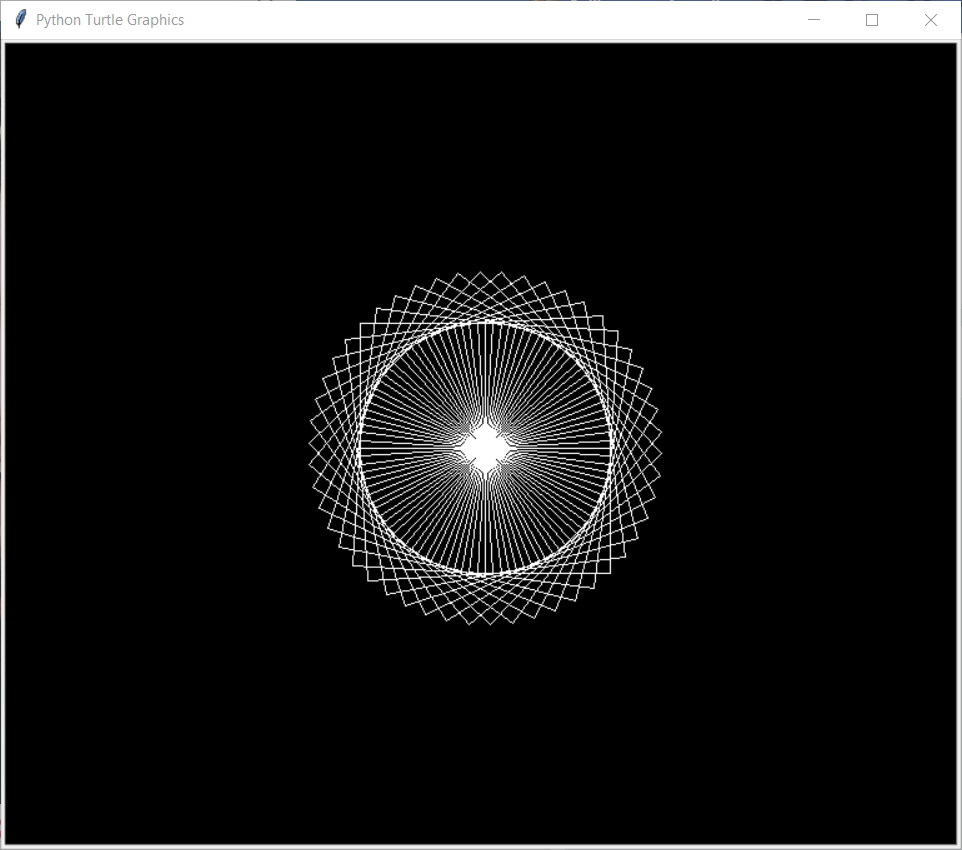
\includegraphics[scale=0.5]{turtle.PNG}
\caption*{Résultat}
\end{center}
\end{figure}

\paragraph{Documentation} \href{https://docs.python.org/fr/3.6/library/turtle.html#methods-specific-to-screen-not-inherited-from-turtlescreen}{Documentation Python 3}, \href{https://fr.wikibooks.org/wiki/Programmation_Python/Turtle}{Wikilivres}

\section{ctypes}
\index{ctypes}
 Ce module sert à appeler des fonctions écrites en langage C dans des librairies DLL par exemple.
\subsection{Boites de dialogue}
\index{boîte de dialogue}
 Le module ctypes peut servir à faire apparaître des boites de dialogue. On peut modifier le comportement du script Python en fonction du bouton appuyé car la fonction faisant apparaître ces boites renvoie un entier qui dépend du bouton appuyé. Diverses options sont disponibles :
\begin{minted}{python}
# Button styles:
# 0 : OK
# 1 : OK | Annuler
# 2 : Abandonner | Recommencer | Ignorer
# 3 : Oui | Non | Annuler
# 4 : Oui | Non
# 5 : Recommencer | Annuler
# 6 : Annuler | Recommencer | Continuer

# To also change icon, add these values to previous number
# 16 Icone erreur
# 32 Icone question
# 48 Icone attention
# 64 Icone information
\end{minted}

\paragraph{Exemple}
\begin{minted}{python}
ctypes.windll.user32.MessageBoxW(0, "That's an error", "Warning!", 16)
\end{minted}
\begin{figure}[h]
\begin{center}
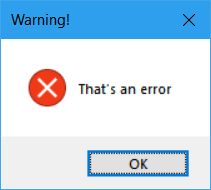
\includegraphics[scale=0.5]{errorwindow.png}
\caption*{Résultat}
\end{center}
\end{figure}

\subsection{keyboard}
\index{keyboard}

\subsection{os}
\index{os}

\subsection{sys}
\index{sys}

\subsection{threading}
index{threading}

\part{Modules à télécharger}
\section{virtualenv}\label{virtualenv}

Les environnement virtuels \marginpar{\href{https://pypi.org/project/virtualenv/}{\mintinline{python}{virtualenv}}} sont un bon moyen pour:
\begin{enumerate}
    \item Installer des modules sans avoir besoin des droits administrateurs
    \item Avoir plusieurs environnements de travail avec des modules Python de versions différentes. Exemple, j'ai un projet Django 2 et je veux créer un site avec Django-CMS, qui requiert Django 1! Je suis obligé de recourir aux environnements virtuels.
\end{enumerate}

Pour une utilisation basique, on commence par installer \mintinline{python}{virtualenv} avec \mintinline{python}{pip}.

\begin{minted}{bash}
$ pip install virtualenv # ou pip3 selon votre version de Python
\end{minted}

Puis on se place dans le dossier où l'on veut placer les environnements virtuels, par exemple sous Linux dans \Verb[fontsize=\small]|/home/votre_nom/python_env/|, et on crée notre environnement!

\begin{minted}{bash}
$ virtualenv env
\end{minted}

Python y place alors les exécutables fondamentaux et quelques modules basiques. Ensuite, pour travailler dans l'environnement créé, il faut lancer la commande:
\begin{minted}{bash}
$ source /home/votre_nom/python_env/env/bin/activate
\end{minted}

L'environnement apparaît maintenant entre parenthèses dans la console. Pour désactiver cet environnement, on lance simplement la commande:

\begin{minted}{bash}
(env) $ deactivate
\end{minted}

Il existe le module \mintinline{python}{virtualenvwrapper}\marginpar{\href{https://pypi.org/project/virtualenvwrapper/}{\texttt{virtualenvwrapper}}} qui permet de naviguer facilement entre les environnements. Après avoir installé ce paquet, il faut ajouter dans le path une variable \mintinline{bash}{WORKON_HOME} qui correspond au répertoire où seront stockés les environnement virtuels. Ensuite on pourra utiliser les commandes

\begin{minted}{bash}
$ mkvirtualenv env # creation d'un environnement virtuel
$ workon # visualisation des environnements existants
env
(env) $ workon env # selection d'un environnement
(env) $ deactivate # quitter cet environnement
\end{minted}

\paragraph{Documentation} \href{https://virtualenv.pypa.io/en/stable/}{Documentation de virtualenv}, \href{http://sametmax.com/les-environnement-virtuels-python-virtualenv-et-virtualenvwrapper/}{informations supplémentaires}


\section{django}
Ce \marginpar{\href{https://pypi.org/project/Django/}{\mintinline{python}{django}}} module permet de créer des sites web en Python. \emph{Il est question ici de la version 2}.
\paragraph{Documentation} \href{https://docs.djangoproject.com/fr/2.0/}{Documentation officielle de Django 2.0} \href{https://docs.djangoproject.com/fr/2.0/intro/}{Tutoriel de la documentation}

\subsection{Fonctionnement}

Django fonctionne selon l'architecture Model-View-Template (MVT) que l'on peut traduire par Modèle-Vue-Gabarit. Celle-ci s’appuie sur l'architecture Model-View-Controler (MVC):
\begin{itemize}
	\item Les modèles structurent de la base de données, là où sont stockées toutes les informations. Ici, ce sont des classes Python dont les attributs correspondent à des champs dans la base de données. On n'écrit jamais de SQL avec Django!
	\item Les vues représentent les pages web: elles présentent les informations aux utilisateurs et récupèrent leurs actions. Ici, ce sont des fonctions Python qui prennent en argument la requête (HTTP par exemple) et des informations sur l’URL et qui renvoie, en utilisant les gabarits, la bonne page à l'utilisateur (la bonne réponse HTTP).
	\item Les gabarits permettent de structurer facilement les vues. Ce sont des fichiers HTML avec un peu de syntaxe de gabarit Django.
	\item Le contrôleur fait l'interface entre les vues et les modèles: il récupère et renvoie les informations nécessaires. Cette partie est gérée de manière autonome par Django.
\end{itemize}

\subsection{Didacticiel}
Cette partie s'appuie sur le tutoriel de la documentation Django, ne pas hésiter à s'y rendre pour plus d'infos. Concertant l'installation, il est conseillé d'installer Django dans un \hyperref[virtualenv]{environnement virtuel}. Dans cet environnement, on utilise l'installateur autonome \mintinline{python}{pip}.

\begin{minted}{bash}
$ pip install Django
\end{minted}

\subsubsection{Créer un projet}
\begin{minted}{bash}
$ django-admin startproject nom_du_projet
\end{minted}

Un dossier est créé, avec trois sous-dossiers (un nommé d'après le projet, un dossier media, et un dossier static) et trois fichiers (une base de données, un fichier python et un fihcier requirements.txt). Pour lancer une première fois le projet sur un serveur local, on utilise la commande (il faut être dans le dossier du projet):
\begin{minted}{bash}
$ python manage.py runserver # on peut remplacer python par python3
\end{minted}
En se rendant sur l’URL indiquée, ou plus simplement \mintinline{python}{localhost:8000} (on peut modifier le port si l'on veut: on écrit le port souhaité à la suite de la commande précédente), on tombe sur une page nous disant que l'installation de Django a réussi.

\subsubsection{Créer une application}
Une fois le projet créé, on crée une première application (cela peut être un sondage, un blog, etc., les applications sont les blocs du site). Une application peut être réutilisée pour d'autres projets. On crée une application par la commande (en étant dans le répertoire du projet) :
\begin{minted}{bash}
$ python manage.py startapp nom_de_l_application
\end{minted}

\subsubsection{Le fichier \mintinline{python}{settings.py}}
Il comporte les principaux paramètres du projet. On y renseigne notamment le type de base de données que l'on utilise; si on utilise SQLite, tout est géré automatiquement. On y gère aussi le fuseau horaire, les langues, les applications installées, parmi les suivantes, installées par défaut:
\begin{itemize}
	\item \mintinline{python}{django.contrib.admin}: l'interface d'administration
	\item \mintinline{python}{django.contrib.auth}: un système d'authentification
	\item \mintinline{python}{django.contrib.contenttypes}: une structure pour les types de contenu
	\item \mintinline{python}{django.contrib.sessions}: un cadre pour les sessions
	\item \mintinline{python}{django.contrib.messages}: un cadre pour l'envoi de messages
	\item \mintinline{python}{django.contrib.staticfiles}: une structure pour la prise en charge des fichiers statiques
\end{itemize}

\subsubsection{Migrations}

Ces applications nécessitent des tables dans la base de données. Elles ne sont pas créées lors de la création du projet (d'où un probable message d'erreur lors du premier lancement), on crée les tables nécessaires grâce à la commande:
\begin{minted}{bash}
$ python manage.py migrate
\end{minted}

Il faut relancer cette commande lorsque l'on doit mettre à jour la base de données, typiquement lorsque l'on crée ou modifie des modèles, ou que l'on importe ou crée des applications.

\subsubsection{Structure des fichiers}
La structure des fichiers est la suivante, pour un projet appelé monsite et une application nommée monapplication.

\begin{minted}{text}
monsite/
    manage.py
    monsite/
        __init__.py
        settings.py
        urls.py
        wsgi.py
    monapplication/
        __init__.py
        admin.py
        migrations/
            __init__.py
        models.py
        tests.py
        views.py
\end{minted}

On s'intéresse maintenant à cette application

\subsubsection{Ecrire une vue}
Les vues s'écrivent dans le fichier \mintinline{python}{views.py}, ce sont des fonctions. On peut commencer par écrire une première vue basique:

\begin{minted}{python}
from django.http import HttpResponse

def index(request):
    return HttpResponse("Hello world!")
\end{minted}

Cette fonction récupère une requette HTTP et renvoie une réponse HTTP. Celle-ci est écrite en HTML ici directement en argument de \mintinline{python}{HttpResponse()}, en général on n'utilise pas cette façon de faire, on utilise les modèles et les gabarits.

\subsubsection{Lui associer une url}
Il faut associer à la vue que l'on vient de créer une URL, c'est-à-dire la requête associée. On crée donc un fichier \mintinline{python}{urls.py} dans le répertoire de l'application:
\begin{minted}{python}
from django.urls import path
from . import views

urlpatterns = [
    path('', views.index, name='index'),
]
\end{minted}

La page \og index \fg{} est par convention (je crois) la page affichée lorsque l'on appelle la racine du projet ou d'une application, c'est pour cela que le premier argument de la fonction \mintinline{python}{path()} est une chaîne vide. Il faut maintenant relier les URL de l'application aux URL du projet, en modifiant \mintinline{python}{urls.py} du répertoire racine du projet:

\begin{minted}{python}
from django.contrib import admin
from django.urls import include
from django.urls import path

urlpatterns = [
    path('monapplication/', include('monapplication.urls')),
    path('admin/', admin.site.urls),
]
\end{minted}

La fonction \mintinline{python}{include()} permet de faire appel aux autres fichiers d’URL que l'on a créés, il faut toujours utiliser cette fonction, la seule exception étant l'administration. On peut tester en lançant un \mintinline{python}{runserver}. Si on va sur \mintinline{python}{localhost:8000}, on a une erreur 404! En se rendant à l'URL \mintinline{python}{localhost:8000/monapplication/ }, Hello world! apparaît.

\subsubsection{Créer un modèle}
Les modèles structurent la base de données et contiennent des métadonnées. Prenons un exemple musical et créons un modèle \mintinline{python}{Artiste} et un modèle \mintinline{python}{Chanson}. On les implémente en tant que classes dans le fichier \mintinline{python}{models.py}:
\begin{minted}{python}
from django.db import models

class Artiste(models.Model):
    nom = models.CharField(max_length=100)
    genre = models.CharField(max_length=100)
    bio = models.TextField(max_length=1000)

class Chanson(models.Model):
    titre = models.CharField(max_length=200)
    annee = models.DateTimeField('année de sortie')
    album = models.CharField(max_length=200)
    artiste = models.ForeignKey(Artiste, on_delete=models.CASCADE)
\end{minted}

Les champs sont représentés par des différentes instance de classe \mintinline{python}{Field}, il en existe divers types. Le premier paramètre non nommé de ces instances permet sert à donner un nom plus lisible à ces champs (ici on l'a utilisé pour \mintinline{python}{annee}).\bigskip

Une fois ces modèles créés, il faut les activer dans la base de données. Pour cela, il faut commencer par indiquer dans le fichier \mintinline{python}{settings.py} que l'on a créé une nouvelle application. On ajoute dans \mintinline{python}{INSTALLED\_APPS} une référence vers la classe de configuration de l'application (qui se trouve dans le fichier \mintinline{python}{apps.py}). On se trouve donc avec, dans \mintinline{python}{settings.py}:

\begin{minted}{python}
INSTALLED_APPS = [
    'monapplication.apps.MonapplicationConfig',
    'django.contrib.admin',
    'django.contrib.auth',
    'django.contrib.contenttypes',
    'django.contrib.sessions',
    'django.contrib.messages',
    'django.contrib.staticfiles',
]
\end{minted}

On indique alors à Django que les modèles ont été modifiés:
\begin{minted}{bash}
$ python manage.py makemigrations monapplication # on n'est pas obligé de mettre le nom de
                                                 # l'application
\end{minted}

Cette instruction est l'analogue d'un \mintinline{python}{git stage}, il faut exécuter ensuite la méthode \mintinline{python}{migrate} pour appliquer les migrations (analogue à \mintinline{python}{git commit}).

\begin{minted}{bash}
$ python manage.py migrate
\end{minted}

\paragraph{Remarque} Les deux étapes précédentes sont à répéter à chaque fois que l'on a modifié les modèles.

\subsubsection{Interface administrateur}
Il y a deux manières d'interagir avec la base de données:
\begin{enumerate}
    \item Avec l'\href{https://docs.djangoproject.com/fr/2.0/topics/db/queries/}{API Django} (non développé ici) à travers le shell Python.
    \item Avec l'interface graphique administrateur de Django.
\end{enumerate}

L'interface administrateur est créée automatiquement. Pour y accéder, il faut commencer par créer un super-utilisateur.

\begin{minted}{bash}
$ python manage.py createsuperuser
\end{minted}

Il suffit ensuite de suivre la procédure. Une fois cela fini, on peut se rendre (après un \mintinline{python}{runserver}) sur l'interface à l'adresse \mintinline{python}{localhost:8000/admin}. Une page de connexion apparaît, on se connecte avec les identifiants du compte super-utilisateur créé précédemment. Après connexion, on arrive sur la page d'administration. Cependant, nous n'avons toujours pas accès aux modèles que l'on a créés. Pour cela, il faut modifier le fichier \mintinline{python}{admin.py} de l'application:
\begin{minted}{python}
from django.contrib import admin
from .models import Chanson
from .models import Artiste

admin.site.register(Artiste)
admin.site.register(Chanson)
\end{minted}
Ainsi, les modèles apparaissent dans un bloc correspondant à l'application concernée (\hyperref[admin2]{figure 1}). On peut donc créer une chanson, par exemple (\hyperref[admin3]{figure 2}). On voit que l'on peut renseigner tous les champs que l'on a créés dans nos modèles. L'outil d’administration est donc un outil très puissant qui nous permet d'agir sur la base de données graphiquement!
\begin{figure}[h]
    \begin{center}
        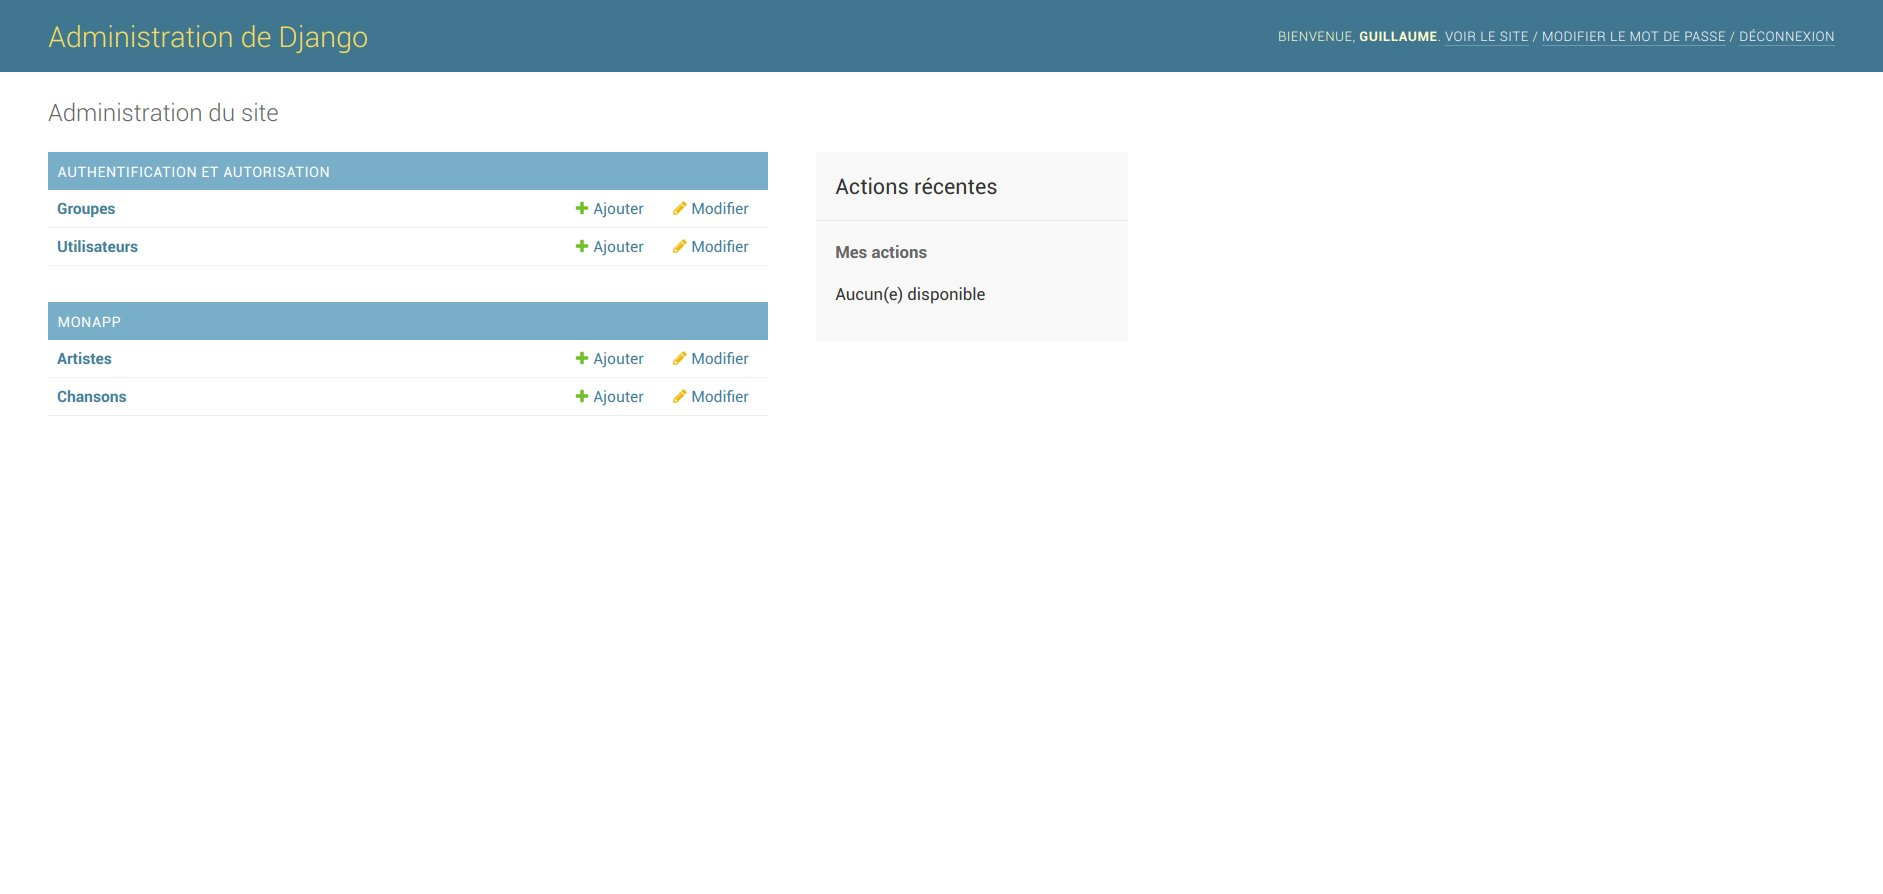
\includegraphics[width=15 cm]{django/admin2.jpg}
        \caption{Administration avec les modèles créés}\label{admin2}
    \end{center}
\end{figure}
\begin{figure}[h]
    \begin{center}
        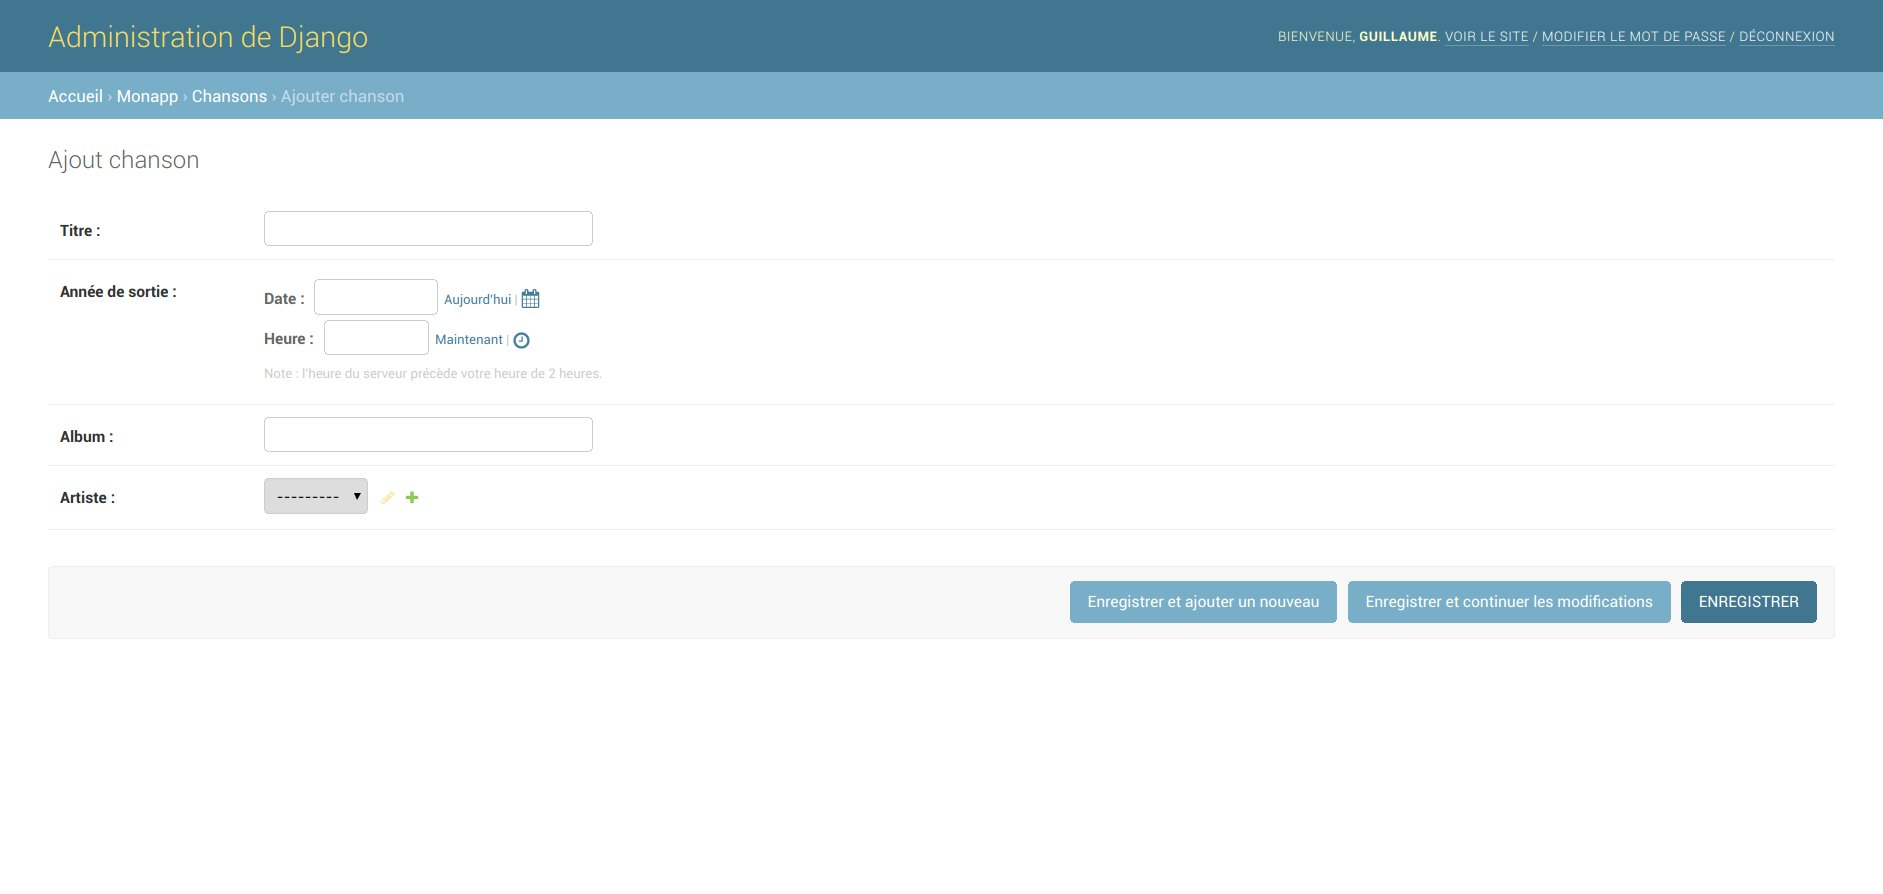
\includegraphics[width=15 cm]{django/admin3.jpg}
        \caption{Créer une chanson}\label{admin3}
    \end{center}
\end{figure}

Si l'on crée une chanson ou un artiste, on peut voir que dans la liste des objets, apparaît la mention "Chanson object" ou bien "Artiste object". En effet, on n'a pas défini de méthode de représentation dans nos modèles, on peut le faire comme suit:
\begin{minted}{python}
from django.db import models

class Artiste(models.Model):
    nom = models.CharField(max_length=100)
    genre = models.CharField(max_length=100)
    bio = models.TextField(max_length=1000)

    def __str__(self):
        return self.nom

class Chanson(models.Model):
    titre = models.CharField(max_length=200)
    annee = models.DateTimeField('année de sortie')
    album = models.CharField(max_length=200)
    artiste = models.ForeignKey(Artiste, on_delete=models.CASCADE)

    def __str__(self):
        return self.titre
\end{minted}

En actualisant la page, les noms des artistes et titres de chansons apparaissent bien.

\subsubsection{Introduction aux vues et gabarits}
Créons plus de vues dans le fichier \mintinline{python}{views.py}. Par exemple des vues qui affichent des artistes et leurs chansons, des vues qui affichent des chansons et leurs paroles. On commence simplement:

\begin{minted}{python}
def artiste(request, artiste_id):
    return HttpResponse("Vous êtes sur la page de l'artiste {}".format(artiste_id))

def chanson(request, chanson_id):
    return HttpResponse("Vous êtes sur la page de la chanson {}".format(chanson_id))
\end{minted}

Il faut ensuite aller renseigner les URL dans \mintinline{python}{urls.py}
\begin{minted}{python}
from django.urls import path
from . import views

urlpatterns = [
    path('', views.index),
    path('chanson/<chanson_id>/', views.chanson),
    path('artiste/<artiste_id>/', views.artiste)
]
\end{minted}

Si on va sur la page \mintinline{python}{localhost:8000/monapplication/artiste/1}, on voit : \og Vous êtes sur la page de l'artiste 1\fg{}. En effet, Django analyse l'URL de la manière suivante:
\begin{enumerate}
    \item \mintinline{python}{monapplication/} il va dans les URL de l’application monapplication
    \item \mintinline{python}{artiste/1/} il cherche la ligne correspondante dans le fichier \mintinline{python}{urls.py}. Il trouve alors la ligne\\ \Verb[fontsize=\small]|artiste/<artiste_id>|, il appelle donc la vue\\ \Verb[fontsize=\small]|artiste(request=<HttpRequest object>, question_id=1)|.
\end{enumerate}

On peut aussi créer des vues qui interagissent avec la base de données en utilisant l'\href{https://docs.djangoproject.com/fr/2.0/topics/db/queries/}{API Django}. Par exemple les pages racines d'artistes et de chansons pourraient les afficher dans l'ordre alphabétique. On aura finalement le fichier \mintinline{python}{views.py} suivant.

\begin{minted}{python}
from django import HttpResponse
from django.shortcuts import render
from .models import Artiste
from .models import Chanson


def index(request):
    return HttpResponse("Hello world!")


def liste_chanson(request):
    liste_chansons = Chanson.objects.order_by('nom')
    context = {
        "liste_chansons": liste_chansons
    }
    return render(request, '/monapplication/chansons/index.html', context)


def liste_artiste(request):
    liste_artistes = Artiste.objects.order_by('nom')
    context = {
        "liste_artistes": liste_artistes
    }
    return render(request, '/monapplication/artistes/index.html', context)


def artiste(request, artiste_id):
    return HttpResponse("Vous êtes sur la page de l'artiste {}"
                        .format(artiste_id))


def chanson(request, chanson_id):
    return HttpResponse("Vous êtes sur la page de la chanson {}"
                        .format(chanson_id))

\end{minted}

On va utiliser des gabarits pour les deux premières vues. La fonction \mintinline{python}{render()} est un raccourci qui permet de renvoyer une réponse HTTP avec un gabarit. Les gabarits sont des fichiers HTML rangés dans le répertoire \mintinline{python}{templates} de l'application. Par exemple pour la liste d'artistes, on aura
\begin{minted}{bash}
monapplication/templates/monapplication/artistes/index.html
\end{minted}

Voici un simple gabarit pour la liste des artistes:
\begin{minted}{html}

    <ul>
    
        <li><a href="/monapp/artiste/{{ artiste.id }}/">{{ artiste.nom }}</a></li>
    
    </ul>

    <p>Aucun artiste.</p>

\end{minted}

\paragraph{Remarque} Même si dans nos modèles, on ne crée pas d'attribut \mintinline{python}{id}, celui-ci est créé automatiquement.\bigskip

Il ne faut pas oublier de mettre à jour \mintinline{python}{urls.py}:
\begin{minted}{python}
urlpatterns = [
    path('', views.index),
    path('chanson/', views.liste_chanson),
    path('artiste/', views.liste_artiste),
    path('chanson/<chanson_id>/', views.chanson),
    path('artiste/<artiste_id>/', views.artiste)
]
\end{minted}

Ainsi, si vous allez sur \mintinline{python}{localhost:8000/artiste/}, la liste de vos artistes s'affichera, ou bien \og Aucun artiste. \fg{} sinon.

\subsubsection{Fichiers statiques}

Les fichiers statiques sont rangés dans un répertoire nommé \mintinline{python}{static}, l'architecture est similaire à celle des gabarits. Imaginons que l'on veuille tout mettre en vert. On crée un fichier \mintinline{python}{style.css} dans le répertoire assoicé à l'application.

\begin{minted}{css}
html {
    color: green;
}
\end{minted}

On modifie ensuite par exemple le gabarit de la liste des artistes en ajoutant ce code au début:
\begin{minted}{html}


<link rel="stylesheet" type="text/css" href="" />
\end{minted}

La balise de gabarit \Verb[fontsize=\small]|| génère l'URL absolue des fichiers statiques. Si on se rend à la page des artistes, tout est vert !

\subsubsection{Thèmes abordés ici}

Cela marque la fin du didacticiel. On s'intéresse maintenant aux différents aspects de Django:
\begin{enumerate}
    \item Les modèles
    \item Les vues
    \item Les gabarits
    \item Les formulaires
    \item L'administration
    \item Le déploiement
\end{enumerate}

Ce n'est pas exhaustif, la meilleure façon de se documenter reste la documentation officielle (qui est d'ailleurs très bien faite).

\subsection{Les modèles et les opérations sur la base de données}

Comme \marginpar{\href{https://docs.djangoproject.com/fr/2.0/ref/models/}{\mintinline{python}{django.db.models}}} indiqué dans le didacticiel:
\begin{enumerate}
    \item Les modèles sont des classes filles de \mintinline{python}{models.Model} que l'on écrit dans le fichier \mintinline{python}{models.py} de l'application concernée.
    \item Cette application doit être mentionnée dans la liste \mintinline{python}{INSTALLED\_APPS} du fichier \mintinline{python}{settings.py}
    \item Un modèle correspond à une table de la base de données. Les champs sont les attributs de la classe du modèle.
\end{enumerate}

\paragraph{Documentation} \href{https://docs.djangoproject.com/fr/2.0/topics/db/}{Documentation Django 2 --- Portail thématique sur les modèles}

\subsubsection{Les champs: attributs des modèles}

Un champ \marginpar{\href{https://docs.djangoproject.com/fr/2.0/ref/models/fields/\#field-types}{\mintinline{python}{models.Field}}} de modèle doit être une instance de la classe \mintinline{python}{Field} (où l'une de ses dérivées). Le choix du type de champ détermine le genre de donnée à stocker (par exemple des nombres ou du texte), le composants HTML qui sera utilisé dans le formulaire utilisé pour renseigner ce champs dans l'administration, et enfin les exigences minimales de validation de ce champ. Se référer aux liens dans la marge pour une documentation complète. Quelques types de champs génériques:
\begin{description}
    \item[\mintinline{python}{class CharField(max_length=None, **options)}]~

    Un champ pour une chaîne de caractère (courte ou longue). Le paramètre \mintinline{python}{max\_length} règle la taille maximale de ce champ. Il en existe de plus précis pour les mails ou les URL, cf. la doc.

    \item[\mintinline{python}{class DateField(auto_now=False, auto_now_add=False, **options)}]~

    Une date, représentée par la classe Python \hyperref[datetime]{\mintinline{python}{datetime.date}}. Le paramètre \mintinline{python}{auto\_now} permet d'assigner automatiquement la date du jour à chaque enregistrement de l'objet, tandis que \mintinline{python}{auto\_now\_add} enregistre la date du jour à la création de l'objet.

    \item[\mintinline{python}{class DateTimeField(auto_now=False, auto_now_add=False, **options)}]~

    Une heure, représentée par la classe Python \mintinline{python}{datetime.datetime}

    \item[\mintinline{python}{class IntegerField(**options)}]~

    Un nombre entier compris entre -2147483648 et 2147483647.

    \item[\mintinline{python}{class TextField(**options)}]~

    Un champ de texte, plus adapté que \mintinline{python}{CharField} pour les longs textes, car la zone de saisie est plus importante dans le formulaire (on ne détaille pas ici les composants HTML de formulaires, cf. la doc)
\end{description}

\subsubsection{Les relations entre les modèles}

On \marginpar{\href{https://docs.djangoproject.com/fr/2.0/ref/models/fields/\#module-django.db.models.fields.related}{\mintinline{python}{models.ForeignKey}}} peut aussi renseigner les relations entre les modèles (donc entre les tables de la base de données).
\begin{description}
    \item[\mintinline{python}{class ForeignKey(to, on_delete, **options)}]~

    Une relation plusieurs-à-un, (cf. le didacticiel, exemple des chansons qui ont l'artiste en \mintinline{python}{ForeignKey}). Cette classe exige la classe à laquelle le modèle et relié, et l'option \mintinline{python}{on\_delete}: \mintinline{python}{models.CASCADE} si l'on veut que lorsque l'on supprime la \mintinline{python}{ForeignKey}, que tous les objets associés du modèle concerné soient supprimés, ou bien \mintinline{python}{SET\_NULL} si l'on veut que les objets aient la valeur \mintinline{python}{null} à la place de la \mintinline{python}{ForeignKey} supprimée (dans ce cas il faut aussi renseigner \mintinline{python}{null=True}). Il y a d'autres possibilités (cf. la doc), \href{https://docs.djangoproject.com/fr/2.0/topics/db/examples/many_to_one/}{voir des exemples}.

    \item[\mintinline{python}{class OneToOneField(to, on_delete, parent_link=False, **options)}]~

    Une relation un-à-un, dont le fonctionnement est similaire à \mintinline{python}{ForeignKey}; \href{https://docs.djangoproject.com/fr/2.0/topics/db/examples/one_to_one/}{voir des exemples}.

    \item[\mintinline{python}{class ManyToManyField(to, **options)}]~

    Une relation plusieurs-à-plusieurs, qui fonctionne de la même manière que \mintinline{python}{ForeignKey} (avec d'autres paramètres supplémentaires, cf. la doc); \href{https://docs.djangoproject.com/fr/2.0/topics/db/examples/many_to_many/}{voir des exemples}.
\end{description}

\subsubsection{Les options des champs}
Les champs acceptent des \mintinline{python}{options}\marginpar{\href{https://docs.djangoproject.com/fr/2.0/ref/models/fields/\#field-options}{\mintinline{python}{**options}}}, en voici quelques unes (on note après un signe \mintinline{python}{=} la valeur par défaut):
\begin{description}
    \item[\mintinline{python}{null=False}]~

    Si la valeur est \mintinline{python}{True}, alors Django stocke les valeurs vides dans la base de données avec \mintinline{python}{NULL}.

    \item[\mintinline{python}{blank=False}]~

    Si la valeur est \mintinline{python}{True}, alors on peut laisser ce champ vide (cette option agit lors de la validation, ne pas confondre avec le paramètre précédent).

    \item[\mintinline{python}{choices}]~

    C'est un itérable (tuple ou liste par exemple) constitué de couples \mintinline{python}{(A, B)} où \mintinline{python}{A} est la valeur réelle pour le modèle et \mintinline{python}{B} le texte affiché à l'utilisateur. On peut organiser en sous groupe comme dans cet exemple:

    \begin{minted}{python}
choix_media = [
    ['Audio', [('vinyl', 'Vinyl'), ('cd', 'CD')]],
    ['Vidéo', [('vhs', 'Cassette VHS'), ('dvd', 'DVD')]],
    ('unknown', 'Unknown'),
]
    \end{minted}

    \item[\mintinline{python}{default}]~

    C'est la valeur par défaut du champ, cela peut être un objet ou un objet exécutable (dans ce cas, il est appelé lors de la création de l'objet). Il ne peut pas s'agir d'un objet muable! En effet, le système de noms de Python ferait que plusieurs instances de modèles seraient référencés vers une même instance de cet objet. Au lieu de cela, on crée une fonction qui retourne cet objet muable.

    \item[\mintinline{python}{help_text}]~

    C'est une chaîne de caractère qui décrit le champ concerné, utilise lorsque l'on utilise la documentation générée automatiquement par Django.

    \item[\mintinline{python}{primary_key}]~

    Si la valeur est \mintinline{python}{True}, alors ce champ représentera une clé primaire du modèle. Si aucun champ n'est renseigné, Django en crée un automatiquement: \mintinline{python}{id}.

    \item[\mintinline{python}{verbose_name}]~

    Chaîne de caractère qui est le \og nom verbeux \fg{} de l'attribut, c'est-à-dire un nom humainement compréhensible pour cet attribut. Il sera affiché à la place du nom de l'attribut dans le formulaire de l'administration (Django l'utilise en convertissant les soulignés en espaces). A l'exception des champs de relations, ce nom verbeux peut-être renseigné en tant que premier paramètre non nommé du champ. Pour ces exceptions, on doit nommer cette option.
\end{description}

\subsubsection{Les métadonnées}
On \marginpar{\href{https://docs.djangoproject.com/fr/2.0/ref/models/options/}{\mintinline{python}{Meta}}} peut attribuer des métadonnées à un modèle grâce à une classe \mintinline{python}{Meta} incorporée dans la classe du modèle. C'est une classe facultative. Elle permet d'enrichir l'interface administrateur. On y renseigne plusieurs options, en voici quelques unes:
\begin{description}
    \item[\mintinline{python}{ordering="-order_date"}]~

    Définit une méthode de tri des instances d'un modèle. C'est une liste ou un tuple de chaîne de caractères. Chaque chaîne correspond à un nom de champ, préfixé par un \mintinline{python}{-} si l'on veut que le tri soit descendant (on ne met rien pour un tri ascendant). Les tris sont rangés dans la liste par ordre de priorité (Django trie par rapport au premier critère, puis second, etc.)

    \item[\mintinline{python}{verbose_name}, \mintinline{python}{verbose_name_plural}]~

    Noms verbeux (même principe que pour les champs) respectivement dans le cas du singulier et dans le cas du pluriel.

    \item[\mintinline{python}{db_table}]~

    Nom de la table dans la base de données. Par défaut, Django la nomme \mintinline{python}{application\_modèle}.
\end{description}

\subsubsection{Les gestionnaires}
Le gestionnaire \marginpar{\href{https://docs.djangoproject.com/fr/2.0/topics/db/managers/}{\mintinline{python}{models}}\par\quad\href{https://docs.djangoproject.com/fr/2.0/topics/db/managers/}{\mintinline{python}{.manager}}\par\quad\quad\href{https://docs.djangoproject.com/fr/2.0/topics/db/managers/}{\mintinline{python}{.Manager}}} est l'interface par laquelle on fait des requêtes à la base de données avec l'\href{https://docs.djangoproject.com/fr/2.0/topics/db/queries/}{API Django} (voir le didacticiel pour un exemple, dans les vues \mintinline{python}{liste\_artistes} ou \mintinline{python}{liste\_chansons}. Le gestionnaire permet aussi bien d'inspecter la base de données que de la modifier.

\begin{description}
    \item[\mintinline{python}{class Manager}]~

    Gestionnaire de la classe concernée. Par défaut, on a (on ne l'écrit pas mais c'est comme-ci):
    \begin{minted}{python}
class Modèle:
    # ...
    objects = models.Manager()
    \end{minted}

    On peut définir un gestionnaire personnalisé (par exemple pour une classe \mintinline{python}{Personne}, on peut le nommer \mintinline{python}{personnes}), dans ce cas, \mintinline{python}{Modèle.objects} produira une exception \mintinline{python}{AttributeError}. Si l'on veut définir un gestionnaire avec des méthodes personnalisées, il suffit de créer une classe héritant de \mintinline{python}{Manager}.
\end{description}

\subsubsection{Modifier la base de données}
L'administration \marginpar{\mintinline{python}{models}\par\quad\mintinline{python}{.base}\par\quad\quad\href{https://docs.djangoproject.com/fr/2.0/ref/models/instances/}{\mintinline{python}{.Model}}} permet de facilement modifier la base de données à la main, mais on doit utiliser l'API Django si on veut modifier la base de données à partir des vues ou des modèles eux-mêmes (par exemple, en reprenant l'exemple du didacticiel, on peut imaginer que la sauvegarde d'un objet Chanson dans la base de données entraînera la création et sauvegarde de l'objet Artiste associé s'il n'existe pas).\bigskip

Pour insérer un objet dans la table de données, on commence déjà par l'instancier. Comme indiqué dans le didacticiel, tous les modèles héritent de la classe \mintinline{python}{Model}.

\begin{description}
    \item[\mintinline{python}{class Model}]~

    Tous les modèles doivent hériter de cette classe! Ainsi on a accès à toutes les méthodes définies par défaut. Il est déconseillé de surcharger l'initialiseur \mintinline{python}{__init__}, car cela pourrait entraîner des erreurs. Il est conseillé de créer un gestionnaire personnalisé (une classe qui hérite de \mintinline{python}{Manager}) et d'y écrire la méthode personnalisée.
\end{description}

Une fois les objets créés, on peut modifier leurs attributs (donc leurs futurs champs). Pour les inclure dans la base de données, il faut les sauvegarder. La première étape consiste à valider l'instance.

\begin{description}
    \item[\mintinline{python}{Model.clean_fields(self, exclude=None)}]~

    Cette méthode valide les champs de l'instance (typiquement, lève une erreur si un champ est vide, alors qu'on n'a pas le paramètre \mintinline{python}{blank=True}). L'option \mintinline{python}{exclude} permet d'indiquer des champs à ignorer lors de la validation. Si la validation échoue, lève une exception \mintinline{python}{ValidationError}.

    \item[\mintinline{python}{Model.clean(self)}]~

    Une méthode à personnaliser pour effectuer des méthodes personnalisées sur notre modèle (effectuer automatiquement des valeurs à des champs, effectuer des validations qui demandent de vérifier plusieurs champs simultanément par exemple). Devrait lever une exception \mintinline{python}{ValidationError} si échoue.

    \item[\mintinline{python}{Model.validate_unique(self, exclude=None)}]~

    Vérifie les contraintes d'unicité du modèle et lève une \mintinline{python}{ValidationError} si échoue.

    \item[\mintinline{python}{Model.full_clean(self, exclude=None, validate_unique=True)}]~

    Exécute les trois méthodes précédentes (exécute \mintinline{python}{validate\_unique} si le paramètre correspondant est \mintinline{python}{True}).
\end{description}

\subsubsection{Récupérer des informations de la base de données}
Lorsque \marginpar{\href{https://docs.djangoproject.com/fr/2.0/ref/models/querysets/}{\mintinline{python}{models}}\par\quad\href{https://docs.djangoproject.com/fr/2.0/ref/models/querysets/}{\mintinline{python}{.query}}\par\quad\quad\href{https://docs.djangoproject.com/fr/2.0/ref/models/querysets/}{\mintinline{python}{.QuerySet}}} l'on veut récupérer des informations de la base de données, on utilise l'API Django. Différentes méthodes appliquées sur les gestionnaires des modèles permettent d'obtenir des objets \mintinline{python}{QuerySet} qui contiennent les informations désirées. En résumé, on utilise la syntaxe:
\begin{minted}{python}
# schéma
query_set = Modèle.gestionnaire.methode()
# exemple
liste_artistes = Artiste.objects.all() #  objects est le nom par défaut du gestionnaire
# on peut aussi appeler ces méthodes sur des QuerySet
liste_artistes_inversee = liste_artistes.reverse()
\end{minted}
 Voici quelques méthodes qui renvoient un \mintinline{python}{QuerySet}:

\begin{description}
    \item[\mintinline{python}{gestionnaire.all()}]~

    Renvoie un \mintinline{python}{QuerySet} contenant toutes les entrées de la table.

    \item[\mintinline{python}{gestionnaire.filter(**kwargs)}]~

    Renvoie un \mintinline{python}{QuerySet} contenant tous les objets répondant aux \href{https://docs.djangoproject.com/fr/2.0/ref/models/querysets/#field-lookups}{paramètres rentrés}.

    \item[\mintinline{python}{gestionnaire.exclude(**kwargs)}]~

    Renvoie un \mintinline{python}{QuerySet} contenant tous les objets sauf ceux répondant aux \href{https://docs.djangoproject.com/fr/2.0/ref/models/querysets/#field-lookups}{paramètres rentrés}.

    \item[\mintinline{python}{gestionnaire.reverse(**kwargs)}]~

    Renvoie le \mintinline{python}{QuerySet} dans l'ordre inverse.

    \item[\mintinline{python}{gestionnaire.distinct(**kwargs)}]~

    Renvoie un \mintinline{python}{QuerySet} sans doublon.
\end{description}

Il y a plusieurs façons d'exploiter un \mintinline{python}{QuerySet}:
\begin{itemize}
    \item Ils sont itérables:
    \begin{minted}{python}
# On imagine qu'on a déjà un QuerySet, on reprend le modèle du didacticiel
>>> liste_artistes
<QuerySet [<Artiste: Muse>, <Artiste: Keane>, <Artiste: Imagine Dragons>]>
>>> for artiste in liste_artistes:
...    print(artiste.nom)
...
Muse
Keane
Imagine Dragons
    \end{minted}

    \item On peut facilement récupérer le nombre d'éléments
    \begin{minted}{python}
>>> len(liste_artistes)
3
    \end{minted}

    \item On peut convertir le \mintinline{python}{QuerySet} en liste:
    \begin{minted}{python}
>>> L = list(liste_artistes)
>>> L
[<Artiste: Muse>, <Artiste: Keane>, <Artiste: Imagine Dragons]
    \end{minted}

    \item Il existe des méthodes qui évaluent un \mintinline{python}{QuerySet} et qui renvoient autre chose qu'un \mintinline{python}{QuerySet}. En voici quelques unes.

    \begin{description}
        \item[\mintinline{python}{query_set.get(**kwargs)}]~

        Renvoie \emph{l'unique} objet répondant aux paramètres rentrés. S'il existe plusieurs objets possibles, ou zéro objet possible, cette fonction renvoie une erreur (respectivement \mintinline{python}{MultipleObjectsReturned} et \mintinline{python}{DoesNotExist}). Si une requête renvoie un \mintinline{python}{QuerySet} singleton, on peut directement récupérer l'objet avec cette méthode sans paramètre (c'est risqué).

        \item[\mintinline{python}{query_set.get_or_create(defaults=None, **kwargs)}]~

        Même comportement que ci-dessus, sauf que si l'objet n'existe pas, il est créé. Renvoie un tuple \mintinline{python}{objet, créé} où \mintinline{python}{objet} est l'objet créé ou charge, \mintinline{python}{créé} un booléen: \mintinline{python}{True} si l'objet a été créé et \mintinline{python}{False} sinon. Cette méthode permet d'alléger la syntaxe et d'éviter d'avoir recours à \mintinline{python}{try: ... except: ...}. Les méthodes permettant d'agir sur la base de données sont détaillées plus loin.

        \item[\mintinline{python}{query_set.update_or_create(defaults=None, **kwargs)}]~

        Essaie de trouver un objet correspondant aux paramètres et lui assigne les nouvelles valeurs rentrées, et crée l'objet s'il n'existe pas. Renvoie la même chose que la méthode précédente.

        \item[\mintinline{python}{query_set.last()}]~

        Renvoie le dernier objet d'un \mintinline{python}{QuerySet} (si ce dernier n'est pas trié, il est automatiquement trié selon la clé primaire).

        \item[\mintinline{python}{query_set.first()}]~

        Idem que la méthode précédente mais renvoie le premier objet.

        \item[\mintinline{python}{query_set.latest(*fields)}]~

        Renvoie l'objet le plus récent selon le champ indiqué (on les indique de la même manière que pour \mintinline{python}{ordering}).

        \item[\mintinline{python}{query_set.earliest(*fields)}]~

        Idem que la méthode précédente mais renvoie le plus ancien.

    \end{description}
\end{itemize}

\subsection{Les requêtes HTTP: vues et URL}
Comme \marginpar{\href{https://docs.djangoproject.com/fr/2.0/ref/request-response/}{\mintinline{python}{django.http}}}indiqué dans le didacticiel:
\begin{enumerate}
    \item Les vues sont des fonctions, rangées dans le fichier \mintinline{python}{views.py} de l'application.
    \item Elles prennent en paramètre obligatoirement une requête Web (à laquelle peuvent s'ajouter des paramètres facultatifs) et renvoient une réponse Web.
    \item La gestion des URL associées aux vues se fait dans le fichier \mintinline{python}{urls.py}.
\end{enumerate}

\paragraph{Documentation} Documentation Django 2 --- \href{https://docs.djangoproject.com/fr/2.0/topics/http/views/}{Ecriture des vues} ---  \href{https://docs.djangoproject.com/fr/2.0/topics/http/urls/}{Distribution des URL}

\subsubsection{Requêtes HTTP}
Les \marginpar{\href{https://docs.djangoproject.com/fr/2.0/ref/request-response/\#httprequest-objects}{\mintinline{python}{http.HttpRequest}}} vues manipulent des requêtes HTTP et renvoient une réponse HTTP en utilisant les modèles et les gabarits. Elles prennent en paramètres une requête HTTP et d'éventuels paramètres supplémentaires dans l'URL (cf. le didacticiel). On commence par décrire ce qu'est une requête HTTP pour Django.

\begin{description}
    \item[\mintinline{python}{class HttpRequest}]~

    Lorsque Django reçoit une requête HTTP, il crée une instance de cette classe contenant les métadonnées associées à la requête. Elle est ensuite mise en premier paramètre de la vue appropriée (ce paramètre est par convention nommé \mintinline{python}{request}, cf. les exemples dans le didacticiel). Cette classe présente plusieurs attributs et méthodes (voir la doc).
\end{description}

\subsubsection{Réponse HTTP}
On \marginpar{\href{https://docs.djangoproject.com/fr/2.0/ref/request-response/\#httpresponse-objects}{\mintinline{python}{http.HttpResponse}}} s'intéresse maintenant à ce que les vues renvoient: les réponses HTTP.

\begin{description}
    \item[\mintinline{python}{class HttpResponse}]~

    Cette classe hérite de \mintinline{python}{HttpResponseBase}. Les réponses HTTP ne sont pas créées automatiquement par Django, ce sont les vues qui les créent. \emph{Une vue se doit de retourner une réponse HTTP!} Typiquement, on peut créer une réponse HTTP avec comme unique paramètre une chaîne de caractère qui sera le contenu de la page HTML retournée.

    \begin{minted}{python}
response = HttpResponse("Voici du texte de page Web.")
    \end{minted}

    Quelques attributs:

    \begin{description}
        \item[\mintinline{python}{HttpResponse.content}]~

        Une chaîne de caractères qui représente le contenu de la réponse.

        \item[\mintinline{python}{HttpResponse.status_code}]~

        Code HTTP de la réponse, 200 par défaut (succès de la réponse). Des classes filles de \mintinline{python}{HttpResponse} ont une valeur par défaut différente.
    \end{description}

    Il existe aussi diverses méthodes (cf. la doc).

    \item[\mintinline{python}{class HttpResponseNotFound(HttpResponse)}]~

    Exemple de classe fille de \mintinline{python}{HttpResponse}, identique à sa classe mère à l'exception de son code HTTP, ici, 404. Il en existe d'autres (voir la doc).
\end{description}

Comme \marginpar{\href{https://docs.djangoproject.com/fr/2.0/topics/http/shortcuts/\#render}{\mintinline{python}{django}}\par\quad\href{https://docs.djangoproject.com/fr/2.0/topics/http/shortcuts/\#render}{\mintinline{python}{.shortcuts}}\par\quad\quad\href{https://docs.djangoproject.com/fr/2.0/topics/http/shortcuts/\#render}{\mintinline{python}{.render}}} premier paramètre (c'est-à-dire \mintinline{python}{content}), on peut utiliser une méthode de gabarit, la méthode \mintinline{python}{render}, qui permet de renvoyer du HTML en utilisant les gabarits. Il existe le raccourci \mintinline{python}{render} pour alléger le code:

\begin{description}
    \item[\mintinline{python}{render(request, template_name, context=None, content_type=None, status=None, using=None)}]~

    Fonction qui combine un gabarit avec dictionnaire de contexte et renvoie une \mintinline{python}{HttpResponse} avec le texte résultant. Deux paramètres obligatoires: \mintinline{python}{request} et \mintinline{python}{template\_name}, le nom complet du gabarit à utiliser.
\end{description}

Les deux vues suivantes sont équivalentes (issus de la doc
 Django):
\begin{minted}{python}
from django.shortcuts import render
from .models import Question

def index(request):
    latest_question_list = Question.objects.order_by('-pub_date')[:5]
    context = {'latest_question_list': latest_question_list}
    return render(request, 'polls/index.html', context)
\end{minted}

\begin{minted}{python}
from django.http import HttpResponse
from django.template import loader
from .models import Question

def index(request):
    latest_question_list = Question.objects.order_by('-pub_date')[:5]
    template = loader.get_template('polls/index.html')
    context = {
        'latest_question_list': latest_question_list,
    }
    return HttpResponse(template.render(context, request))
\end{minted}


\subsubsection{La gestion des URL}
Les URL \marginpar{\href{https://docs.djangoproject.com/fr/2.0/ref/urls/}{\mintinline{python}{django.urls}}} (Uniforme Resource Locators) sont gérés dans les différents fichiers \mintinline{python}{urls.py}. Il y en a un dans chaque application et un dans le répertoire racine. Les URL sont configurées dans la liste \mintinline{python}{urlpatterns}. Voici les principales fonctions à utiliser.

\begin{description}
    \item[\mintinline{python}{path(route, view, kwargs=None, name=None)}]~

    Cette fonction est utilisée dans la liste \mintinline{python}{urlpatterns}. Elle prend deux paramètres obligatoires: la route, une chaîne de caractère qui correspond à une URL, et une vue (ou bien la fonction \mintinline{python}{include} qui appelle d'autres URL). La route peut contenir des éléments entre chevrons \mintinline{python}{<paramètre>} qui servent de paramètres pour la vue (rappel: les vues sont des fonctions).

    \item[\mintinline{python}{include(module, namespace=None)}]~

    Cette fonction, en général utilisée comme second paramètre de la fonction \mintinline{python}{path()} prend en argument un module d'URL qu'il faut inclure après l'URL mise en premier paramètre.
\end{description}


\subsection{Les gabarits}
Un gabarit Django est un fichier texte ou une chaîne de caractères Python balisée en utilisant le langage de gabarit Django. Certaines expressions (étiquettes et variables) sont reconnues et inerprétées par le moteur de gabarit. Pour rendre un gabarit, celui-ci a besoin d'un dictionnaire de contexte: il remplace les variables par leur valeur et exécute les étiquettes. Le reste est maintenu tel quel.

\paragraph{Documentation} \href{https://docs.djangoproject.com/fr/2.0/topics/templates/}{Documentation Django 2}


\subsubsection{La syntaxe des gabarits}
\paragraph{Les variables}
Elles utilisent le dictionnaire de contexte pour afficher leur valeur correspondante. Les noms des variables sont les clés du dictionnaire. Dans le gabarit, les variables sont entourées de doubles accolades: \mintinline{python}{\{\{} et \mintinline{python}{\}\}}. Par exemple, le gabarit
\begin{minted}{text}
La chanson {{ chanson }} a été écrite par {{ artiste }}.
\end{minted}
avec le dictionnaire \mintinline{python}{\{'artiste': 'Muse', 'chanson': 'Starlight'\}} donnera:
\begin{minted}{text}
La chanson Starlight a été écrite par Muse.
\end{minted}

On accèdes aux attributs d'instances, aux indices de listes, aux clés de dictionnaires par une notation pointée.
\begin{minted}{text}
{{ dico.clé }}
{{ objet.attribut }}
{{ liste.indice }}
\end{minted}

Si la valeur de la variable est une fonction (ou n'importe quel objet exécutable), il sera appelé sans paramètre et le résultat retourné sera utilisé.

\paragraph{Les balises} Elles \marginpar{\href{https://docs.djangoproject.com/fr/2.0/ref/templates/builtins/\#built-in-tag-reference}{Balises intégrées}}permettent de faire diverses choses, comme utiliser des boucles logiques ou insérer d'autres gabarits. Leur nom sont entourés de \mintinline{python}{\{\%} et \mintinline{python}{\%\}}. Certaines balises sont orphelines, les autres s'utilisent comme ceci:

\begin{minted}{html}
<!-- Exemple de balise nommée balise. -->

<!-- Contenu -->

\end{minted}

\begin{description}
    \item[\mintinline{python}{block}] (oprheline)

    Définit un bloc pouvant être surchargé par des gabarits enfants.

    \item[\mintinline{python}{comment}]~

    Ignore ce qui est compris entre \mintinline{python}{\{\% comment \%\}} et \mintinline{python}{\{\% endcomment \%\}}.

    \item[\mintinline{python}{if}]~

    Evalue une variable et, si celle-ci vaut \mintinline{python}{True} (ie est différent de \mintinline{python}{False}, \mintinline{python}{''} ou \mintinline{python}{None}), affiche le bloc correspondant.

    \begin{minted}{html}

    <!-- contenu -->

    <!-- contenu -->

    <!-- OR est prioritaire sur AND.
    Utiliser des parenthèses est une erreur de syntaxe,
    utiliser des IF imbriqués si nécessaire. -->

    <!-- contenu -->

    <!-- contenu -->

    \end{minted}

    \item[\mintinline{python}{firstof}] (orpheline)

    Affiche le premier paramètre qui ne vaut pas \mintinline{python}{False} et rien dans le cas où aucun paramètre n'est vrai. On peut ajouter un dernier paramètre si aucun n'est validé. On peut utiliser le mot clé \mintinline{python}{as} pour stocker la variable (voir \mintinline{python}{cycle} un peu plus bas).

    \begin{minted}{html}

<!-- est l'équivalent de -->

    {{ var1 }}

    {{ var2 }}

    {{ var3 }}

    "dernier recours"

    \end{minted}

    \item[\mintinline{python}{for}]~

    Effectue une boucle sur chaque élément d'une liste. On peut ensuite utiliser cet élément comme variable. Exemple:
    \begin{minted}{html}
<ul>

    <li>{{ artiste.nom }}</li>

</ul>
    \end{minted}

    On peut ajouter une balise \mintinline{html}{} pour afficher du contenu lorsque la liste est vide (ou n'existe pas).

    \item[\mintinline{python}{cycle}] (orpheline)

    Affiche un de ses paramètres à chaque apparition de la balise: le premier, puis le deuxième, et ainsi de suite; et revient au début lorsque tous les paramètres ont été utilisés. On peut mélanger variables et chaînes de caractères, par exemple:

    \begin{minted}{html}

    <div class="">
        <!-- contenu -->
    </div>

    \end{minted}
    A la première itération, \mintinline{python}{"chaine\_1"} sera utilisé, puis la chaîne contenu dans \mintinline{python}{variable\_de\_la\_chaine\_2}, puis \mintinline{python}{"chaine\_3"}. Il est également possible de sauvegarder temporairement le paramètre dans une variable que l'on peut réutiliser plus loin.

    \begin{minted}{html}

    <div class="">
        <!-- contenu -->
    </div>
    <div class="{{ chaine }}">
    </div>

    \end{minted}

\end{description}

\subsubsection{Utiliser les gabarits dans les vues}


\subsection{Les formulaires}
\paragraph{Documentation} \href{https://docs.djangoproject.com/fr/2.0/topics/forms/}{Documentation Django 2 --- Les formulaires}




\section{twilio}
\index{twilio}
\section{win10toast}
\index{win10toast}
\section{splinter}
\index{splinter}
\section{pylint}
\index{pylint}

\subsection{autopy}
\index{autopy}

\part{Conventions des Python Enhancement Proposals}
\section{PEP 8 : Conventions de style du code Python}
\section{PEP 257 : Convention des docstrings}



%\addcontentsline{toc}{section}{Index}
\printindex
\end{document}
